\documentclass{book}
\usepackage{xeCJK}
\usepackage{titlesec}
%\usepackage[winfonts]{ctex}
\usepackage[all]{xy}
\usepackage{indentfirst}
\usepackage{ntheorem}
\usepackage{amssymb}
\usepackage{amsmath}
\usepackage{amstext}
\usepackage{bussproofs}
\usepackage{changepage}
\usepackage{tikz}
\usepackage{framed}
\usepackage{mdframed}
\titleformat{\chapter}[display]{\Huge\bfseries}{第\,\thechapter\,章}{1em}{}
\titleformat{\part}{\centering\Huge\bfseries}{第\,\thepart\,部分}{1em}{}
\setCJKmainfont[BoldFont=SimHei]{SimSun}
\theoremindent2em
\theorempreskipamount1.5em
\theorempostskipamount1.5em
\parindent=20pt
\parskip=5pt
\def\figoo{\rightsquigarrow\kern-8pt\rightsquigarrow}
\def\v{\mathbf{v}}
\def\r{\mathbf{r}}
\def\n{\mathbf{n}}
\def\R{\mathbf{R}}
\def\lianxi{\noindent \makebox[0pt][r]{$\rhd$} \textbf}
\begin{document}
\part{语言模型}
\chapter{文本求值}
在本书中,我们将学习如何以人们易于理解,同时也适合形式分析的方式定义编程语言——在此,形式分析也应使用人们易于理解的方式。\par
其中一种定义语言的方式是使用文章段落去解释语言中允许的表达式类型以及它们的求值方式。这种方法的优点是读者可以快速掌握语言的核心部分,但是语言的细节却显然难以通过文章段落理解。更糟糕的是,无法用文章段落的方式进行形式分析。\par
另一种定义语言的方式是使用一些元语言来编写这个语言的解释器。如果读者熟悉这种元语言,这种技术显然可以清楚且完整地表示语言细节。如果这种元语言存在形式定义,那么这个解释器同样存在该语言的形式意义,也可以做形式分析。\par
用于定义另一种语言的元语言不必可以高效执行,因为它的首要目的是向人们解释其他语言。元语言的基本数据结构也不必从字和字节的角度定义。实际上,对元语言我们可以直接使用逻辑和基于程序文本全集的集合论。同样,物理机器上的计算也是可以被描述的,最终,从在内存空间中重排列位的角度看,抽象计算也可以从文本关系的角度进行描述。\par
\section{定义集合}
当我们写出如下BNF文法时
\begin{framed}
$$
\begin{array}{lcl}
B & = & t \\
& | & f \\
& | & (B\bullet B)
\end{array}
$$
\end{framed}
实际上则定义了文本串集合$B$。上述的定义可以拓展为B的约束:
$$
\begin{array}{c}
t\in{B}\\
f\in{B}\\
a\in{B}\ \text{且}\ b\in{B}\Rightarrow(a\bullet b)\in{B}
\end{array}
$$
严格的说,B是遵循上述约束的最小集合。\par
注意,我们有时使用“$B$”来代替“集合$B$”,因为通过上下文很容易弄懂其真实的含义。有时在集合名称上使用下标或者撇号表示集合中的任一元素,例如“$B_1$”或者“$B'$”。因此,上面的条件可以写成
$$
\begin{array}{cll}
t\in{B} & \qquad & [a] \\
f\in{B} & \qquad & [b] \\
(B_1\bullet B_2) \in B & \qquad & [c]
\end{array}
$$
无论是用BNF简略表达式定义,还是扩展成约束集进行复杂定义,集合B都是被递归定义的。在有限空间内枚举B的所有元素是不可能的:
$$B=\{t,f,(t\bullet t),(t\bullet f),\ldots\}$$
但是,对B中一段特定文本,通过展示定义B的约束是如果规定属于B的文本,我们可以证明该文本是属于B的。例如,$(t\bullet{(f\bullet{t})})$ 是属于B 的:
$$
\begin{array}{lll}
1.\quad t\in{B} & \qquad & \text{根据}\ [a] \\
2.\quad f\in{B} & \qquad & \text{根据}\ [b] \\
3.\quad t\in{B} & \qquad & \text{根据}\ [a] \\
4.\quad (f\bullet{t})\in{B} & \qquad & \text{根据}\ 2,3,\text{且}[c] \\
5.\quad (t\bullet (f\bullet{t}))\in{B} & \qquad & \text{根据}\ 1,4,\text{且}[c]
\end{array}
$$
我们可以写成证明树形式:
\begin{prooftree}
\AxiomC{$t\in{B}\ [a]$}
\AxiomC{$f\in{B}\ [b]$}
\AxiomC{$t\in{B}\ [a]$}
\BinaryInfC{$(f\bullet t)\in B\qquad[c]$}
\BinaryInfC{$(t\bullet (f\bullet t))\in B\qquad\qquad[c]$}
\end{prooftree}
我们也可以省略证明树上被应用规则的名称,因为这通常是显而易见的:
\begin{prooftree}
\AxiomC{$t\in{B}$}
\AxiomC{$f\in{B}$}
\AxiomC{$t\in{B}$}
\BinaryInfC{$(f\bullet t)\in B$}
\BinaryInfC{$(t\bullet (f\bullet t))\in B$}
\end{prooftree}
\lianxi{练习1.1.} 下面哪个是属于B的?为B中的每个元素都写出一个以证明该元素一定属于B的证明树。
\begin{enumerate}
 \item t
 \item $\bullet$
 \item $((f\bullet t)\bullet(f\bullet f))$
 \item $((f)\bullet(t))$
\end{enumerate}

\section{关系}
关系是由有序对\footnote{有序对$\langle x,y\rangle$可以表示成$\{\{x\},\{x,y\}\}$的集合}构成的集合。例如,我们可以定义关系$\equiv$去让每个$B$中的元素和它自身匹配:
$$
a\in{B}\quad\Rightarrow\quad\langle{a,a}\rangle\in\equiv
$$
对类似$\equiv$的二元关系,我们通常写成$a\equiv a$而不是$\langle{a,a}\rangle\in\equiv$。
$$a\in{B}\quad\Rightarrow\quad a\equiv a$$
或者更简单的
$$B_1\equiv B_1$$
只要该表达式可以被理解为$\equiv$的定义。事实证明,关系$\equiv$是自反的、对称的和传递的。
$$
\begin{array}{ll}
\mbox{关系$\mathbf{R}$是\textbf{自反的}当且仅当} & a\ \mathbf{R}\ a\ (\mbox{对任何}a) \\
\mbox{关系$\mathbf{R}$是\textbf{对称的}当且仅当} & a\ \mathbf{R}\ b\Rightarrow b\ \mathbf{R}\ a \\
\mbox{关系$\mathbf{R}$是\textbf{传递的}当且仅当} & a\ \mathbf{R}\ b\ \text{且}\ b\ \mathbf{R}\ c\Rightarrow a\ \mathbf{R}\ c
\end{array}
$$
如果一个关系是自反的,对称的且传递的,那么这个关系也是\textbf{等价的}。\par
下面定义了关系r,既不是自反的,传递的,也不是等价的。
\begin{framed}
$$
\begin{array}{cclc}
(f\bullet{B_1})& \r & B_1 & [a]\\
(t\bullet{B_1})& \r & t & [b]
\end{array}
$$
\end{framed}
根据r,我们可以定义新的关系$\asymp_\r $,且加入一个限制使$\asymp_\r $自反。
$$
\begin{array}{rclc}
(f\bullet{B_1})& \asymp_\r  & B_1 & [a]\\
(t\bullet{B_1})& \asymp_\r  & t & [b]\\
B_1 &  \asymp_\r  & B_1 & [c]
\end{array}
$$
关系$\asymp_\r $是r的\textbf{自反闭包},我们可以加入对称和传递限制来构造一个新的关系:
$$
\begin{array}{rclc}
(f\bullet{B_1})& \approx_\r  & B_1 & [a]\\
(t\bullet{B_1})& \approx_\r  & t & [b]\\
B_1 &  \approx_\r  & B_1 & [c]\\
B_1 \approx_\r  B_2 & \Rightarrow & B_2 \approx_\r  B_1 & [d]\\
B_1 \approx_\r  B_2\ \text{且}\ B_2 \approx_\r  B_3 &  \Rightarrow & B_1 \approx_\r  B_3  & [e]
\end{array}
$$
$\approx_\r $是$\asymp_\r $的\textbf{对称传递闭包},也是r的\textbf{自反对称传递闭包}或者\textbf{等价闭包}。
\section{求值关系}
B和r的实例应该能让你理解编程语言是如何通过文本和基于文本的关系定义的,或者更准确的说,是如何通过集合$(B)$和基于集合$(r)$的关系定义的。\par
事实上,你也许开始猜测B是布尔表达式的文法,其中$\bullet$对应“or”,$\approx_\r $等同于含有相同布尔值的表达式。\par
实际上,基于上述约束,我们可以证明$(f\bullet t)\approx_\r (t\bullet t)$,就像$\mathbf{false}\vee \mathbf{true}=\mathbf{true}\vee \mathbf{true}$:
\begin{prooftree}
\AxiomC{$(f\bullet t)\approx_\r  t\ [a]$}
\AxiomC{$(t\bullet t)\approx_\r  t\ [b]$}
\UnaryInfC{$t\approx_\r (t\bullet t)\ [d]$}
\BinaryInfC{$(f\bullet t)\approx_\r (t\bullet t)\qquad[e]$}
\end{prooftree}
但是,这并不表明$\bullet$和“or”完全一致。相反,我们必须证明关于$\bullet$的一般推论,如证明对任何$B_1$有$(B_1\bullet t)\approx_\r  t$(我们很快就会知道,事实上这是不可能被证明的)。\par
换言之,一个解释器定义的语言(即使解释器是用数学语言定义的)和我们可能想要保证的语言性质之间通常存在一定差距。对不同的目的而言,语言的性质和它所计算出的值同样重要。例如,如果$\bullet$真的和“or”行为一致,那么编译器可以安全地将$(B\bullet t)$优化成t。类似的,如果某种语言的语义规则可以保证数值不能和任何非数值相加,那么该语言的实现就不必通过检查加法表达式的参数,来确保二者都是数值。\par
但是,我们首先必须消除定义语言的方式和定义一般求值的方式之间的“元差距”,才能开始处理这些差距。
\section{有向求值}
“求值”规则$\approx_\r $并不完全具有求值的特征。它允许我们证明某些表达式是等价的,却不能告诉我们如何从任意一个$B_1$推导出t或f。\par
从这个角度出发,更简单的关系r是更有效的。r的定义中两种情况都可将一个表达式映射成一个更简洁的表达式。同样,对任意的表达式B,无论B是t或f,r都可以使B关联到最多一个的其他表达式。因此,我们可以认为r是一步规约,对应着解释器对最终结果进行一次可能的单步求值的方式。\par
我们可以定义$\figoo_\r $为r的自反传递闭包,并且最终得到一个\textbf{多步规约}关系。多步关系$\figoo_\r $会将每个表达式映射成多个其他表达式。尽管如此,事实上,$\figoo_\r $会将每个表达式映射成最多一个t或者f。\par
\begin{adjustwidth}{1cm}{1cm}
这足以将$\figoo_\r $定义成“r的自反传递闭包”。像上一节一样,一个交替的公式可以拓展成若干约束。第三种方式是部分拓展现有约束,但需要使用r来定义$\figoo_\r $。
$$
\begin{array}{rcl}
B_1 & \figoo_\r  & B_1 \\
B_1\ \r\ B_2 & \Rightarrow & B_1 \figoo_\r  B_2 \\
B_1 \figoo_\r  B_2\ \text{且}\ B_2 \figoo_\r  B_3 & \Rightarrow & B_1 \figoo_\r  B_3
\end{array}
$$
\end{adjustwidth}\par
关系r和$\figoo_\r $是有意不对称的,相当于需要对一个值向其特定的方向进行求值。例如对表达式$(f\bullet(f\bullet(t\bullet f)))$,我们可以展示一个向t的\textbf{规约}:
$$
\begin{array}{rcl}
(f\bullet(f\bullet(t\bullet f)))\ & \r & (f\bullet(t\bullet f))\\
\ & \r & (t\bullet f) \\
\ & \r & t
\end{array}
$$

左边列的每个空行默认可以被前一行的右侧列补充,然后每一行都是证明$(f\bullet(f\bullet(t\bullet f)))\figoo_\r t$的一步。\\\\
\lianxi{练习1.2.}证明$(f\bullet (f\bullet(f\bullet f)))\figoo_\r f$,通过$\r$的一步关系证明其归约即可。
\section{上下文求值}
表达式$((f\bullet t)\bullet f)$如何规约?根据r或者$\figoo_\r $的约束,它根本不会规约!\par
直觉上,通过$(f\bullet t)\ r\ f$将第一个子表达式简化,$((f\bullet t)\bullet f)$应该规约成$(t\bullet f)$。但是在r的定义中,并没有符合将$ ((f\bullet t)\bullet f)$作为原表达式的约束。我们只能规约形式为$(f\bullet B)$和$(t\bullet B)$的表达式。换句话说,中间$\bullet$右边列的表达式可以是任意的,但是左边列的表达式必须是f或者t。\par
我们可以使用$\rightarrow_\r $拓展关系r以支持子表达式的规约:
\begin{framed}
$$
\begin{array}{rclc}
B_1\ \r\ B_2\quad & \Rightarrow & \quad B_1\rightarrow_\r  B_2 & \quad [a] \\
B_1\rightarrow_\r  B_1' \quad & \Rightarrow & \quad (B_1\bullet B_2)\rightarrow_\r (B_1'\bullet B_2) & \quad [b]\\
B_2\rightarrow_\r  B_2' \quad & \Rightarrow & \quad (B_1\bullet B_2)\rightarrow_\r (B_1\bullet B_2') & \quad [c]
\end{array}
$$
\end{framed}
关系$\rightarrow_\r $是r的\textbf{合拍闭包}。类似r,$\rightarrow_\r $也是一步关系,但是$\rightarrow_\r $允许对整个表达式中任意子表达进行规约。r规约的子表达式称作\textbf{可约项},在\textbf{可约项}周围的文本称作\textbf{上下文}。\par
需要特别指出的是,$\rightarrow_\r $关系包含$((f\bullet t)\bullet f)\rightarrow_\r (t\bullet f)$。我们通过下面的证明树证明这个包含:
\begin{prooftree}
\AxiomC{$(f\bullet t)\ \r\ t$}
\UnaryInfC{$(f\bullet t)\rightarrow_\r  t \  [a]$}
\UnaryInfC{$((f\bullet t)\bullet f)\rightarrow_\r (t\bullet f)\  [b]$}
\end{prooftree}
继续使用关系$\rightarrow_\r $,我们可以规约$((f\bullet t)\bullet f)$到t:
$$
\begin{array}{ccl}
((f\bullet t)\bullet f)&\rightarrow_\r &(t\bullet f)\\
&\rightarrow_\r &t
\end{array}
$$
最后,如果我们定义$\twoheadrightarrow_\r $作为$\rightarrow_\r $的自反传递闭包,我们可以得到$((f\bullet t)\bullet f)\twoheadrightarrow_\r t$。因此,$\twoheadrightarrow_\r $是根据r自然生成的\textbf{规约关系}。\par
总的来说,纯粹的r的自反闭包$\asymp_\r $,等价闭包$\approx_\r $或者自反传递闭包$\figoo_\r $是很乏味的。相反,我们通常会对合拍闭包$\rightarrow_\r $以及它的自反传递闭包$\twoheadrightarrow_\r $感兴趣,因为它们符合经典的求值概念。另外,$\rightarrow_\r $的等价闭包$=_\r $也因关联了相同结果的表达式而耐人寻味。\\\\
\lianxi{练习1.3.}解释为什么$(f\bullet((t\bullet f)\bullet f))\not\figoo_\r t$。\\\\
\lianxi{练习1.4.}通过证明关于$\rightarrow_\r$归约的命题来证明$(f\bullet((t\bullet f)\bullet f))\twoheadrightarrow_\r t$。
\section{求值函数}
虽然$\twoheadrightarrow_\r $让我们更加了解实用的求值概念,但我们仍没有真正的了解它。不仅存在$((f\bullet t)\bullet f)\twoheadrightarrow_\r t$,同样也有$((f\bullet t)\bullet f)\twoheadrightarrow_\r (t\bullet f)$和$((f\bullet t)\bullet f)\twoheadrightarrow_\r ((f\bullet t)\bullet f)$两种情况。\par
对求值而言,我们关心的是B求值成f还是t,任何使用$\twoheadrightarrow_\r $或$=_\r $的映射都与此无关。为了理解求值的概念,我们如下方式定义关系$eval_\r $:
\begin{framed}
$$
eval_\r (B)=
\left\{
\begin{array}{ll}
f & \text{如果$B=_\r f$} \\
t & \text{如果$B=_\r t$}
\end{array}
\right.
$$
\end{framed}
此处我们还是在用另一种概念去定义关系。这种概念让我们联想起\textbf{函数},即将一个元素映射成另一个元素的关系。我们使用函数概念因为$eval_\r $如果想要成为一个求值器则必须先成为一个函数。\\\\
\lianxi{练习1.5.}在$\r,\asymp_\r,\approx_\r,\figoo_\r,\rightarrow_\r,\twoheadrightarrow_\r,=_\r$和$eval_\r$这些关系中,哪些是函数?为每一个非函数关系都找到一个表达式和它关联的两个表达式。
\section{概念汇总}

\begin{tabular}{|cll|}
  \hline
  \textbf{符号} & \textbf{定义} & \textbf{解释}\\
  \hline
  % after \\: \hline or \cline{col1-col2} \cline{col3-col4} ...
  $-$ & 表达式文法中的基本关系 & 没有上下文的一步“规约” \\
  \hline
  $\rightarrow_-$ & 表达式文法\_的合拍闭包 & 上下文的一步规约 \\
  \hline
  $\twoheadrightarrow_-$ & $\rightarrow_-$的自反传递闭包 & 多步规约(0或者多步) \\
  \hline
  $=_-$ & $\twoheadrightarrow_-$的对称传递闭包 & 产生相同结果的等价表达式 \\
  \hline
  $eval_-$ & 限制结果的$=_-$ & 完整的求值 \\
  \hline
\end{tabular}
\chapter{求值的一致性}
既然我们有了结构化指令,我们准备返回到$eval_\r $作为求值器的一致性话题上。换言之,我们想证明$eval_\r $是函数。更加形式化的说,给出结果集R:
$$
\begin{array}{ccc}
R&=&t\\
&|&f
\end{array}
$$
我们想证明如下定理:
\newtheorem{Theorem}{定理}[chapter]
\newtheorem{Lemma}[Theorem]{引理}
\begin{Theorem}
如果$eval_\r (B_0)=R_1$且$eval_\r (B_0)=R_2$,那么$R_1=R_2$。
\end{Theorem}
为了证明该定理,我们假设对某$B_0$、$R_1$和$R_2$,有$eval_\r (B_0)=R_1$且$eval_\r (B_0)=R_2$,而想推出$R_1=R_2$。根据$eval_\r $ 的定义,我们的假设意味着$B_0=_\r R_1$且$B_0=_\r R_2$(使用$=_\r $而非$=$)。因此,根据$=_\r $是等价关系的定义可得$R_1=_\r R_2$。为了得出$R_1=R_2$的结论,我们必须探讨求值的本质,即当$M,N\in B$时,$M=_\r N$证明的一般式。\par
因为$=_\r $是单步规约$\rightarrow_\r $的拓展形式,所以证明$M=_\r N$的求值通常是基于r的一系列单步双向规约:\\
$$
\xymatrix{
  {M} \ar[rd] & & & & & & & {N} \ar[ld] \\
    & {L_1} \ar[rd] & & {L_3} \ar[ld] \ar[rd] & & {\ldots}\ar[ld] &{ L_5}\\
    & & {L_2} & & {L_4} 
}
$$
其中对每个$L_\textbf{n}$有$L_\textbf{n}\in B$。也许这些步骤可以重排,使得所有归约步骤从M到达某个L且从N到达同样的L。换言之,如果$M=_\r N$则可能存在一个表达式L,使$M\twoheadrightarrow_L$且$N\twoheadrightarrow_L$。\par
我们如果可以证明总是存在这样的L,也就完成了一致性的证明。回想我们的断言
$$ R_1=_\r R_2$$
根据该断言(尚未证明),一定存在L使
$$R_1\twoheadrightarrow_\r L\quad \text{且}\quad R_2\twoheadrightarrow_\r L$$
但是R中的元素只有t和f,显然不可能规约成除了他们自身的任何值。所以$L=R_1$且$L=R_2$,意味着$R_1=R_2$。\par
根据前面的论述,我们已经将$eval_\r $的一致性证明规约成证明$M=_\r N$的论据形态的断言。这个关于形式等价系统的一致性证明和规约步骤重排之间的联系的重要见解归功于丘奇和罗瑟,二者将这个思路用于分析称为$\lambda$演算的语言(我们很快会学到)的一致性问题。一般而言,如果一个由基本规约概念按一定条件产生的等价关系满足重排性质,则它满足丘奇罗瑟性质。
\begin{Theorem}[基于$=_\r $的丘奇罗瑟定理]
如果$M=_\r N$,那么存在表达式L使$M\twoheadrightarrow_\r L$且$N\twoheadrightarrow_\r L$。
\end{Theorem}
因为我们有特定的$M=_\r N$,而$=_\r$是递归定义的,所以可以通过对$M=_\r N$的推导结构进行归纳来证明该定理。
\begin{adjustwidth}{20pt}{20pt}
\textbf{定理2.2的证明}:对$M=_\r N$证明结构的归约

\begin{itemize}
  \item 奠基步骤
  \begin{itemize}
    \item \textbf{当}$M\twoheadrightarrow_\r N$\\
    令$L=N$,得证。
  \end{itemize}

  \item 归纳步骤
  \begin{itemize}
    \item \textbf{根据}$N=_\r M$,\textbf{有}$M=_\r N$\\
    根据归纳,L存在于$N=_\r M$,所以该L即为所求。
    \item \textbf{根据}$M=_\r L_0,\ L_0=_\r N$,\textbf{有}$M=_\r N$\\
    根据归纳,存在$L_1$使$M\twoheadrightarrow_\r L_1$且$L_0\twoheadrightarrow_\r L_1$。再次根据归纳,存在$L_2$使$N\twoheadrightarrow_\r L_2$且$L_0\twoheadrightarrow_\r L_2$。如图所示,我们有:
    $$
     \xymatrix{
      {M}\ar[rd] & {=_\r } & {L_0} \ar[ld] \ar[rd] &  {=_\r } & {N} \ar[ld]\\
       & {L_1} & & {L_2}
     }
$$
    现在我们假设,无论$L_0$何时同时规约到$L1$和$L_2$,都存在$L_3$使得$L_1\twoheadrightarrow_\r L_3$且$L_2\twoheadrightarrow_\r L_3$。然后我们想证明的断言即得证,因为$M\twoheadrightarrow_\r L_3$且$N\twoheadrightarrow_\r L_3$。
  \end{itemize}
\end{itemize}
\end{adjustwidth}
我们再一次完成了这个证明,但留下了另一个关于归约系统的断言有待证明。这个新性质叫做\textbf{菱形性质},因为这个定理的形状需要规约能按照菱形排列:
$$
 \xymatrix{
   & {L} \ar[ld] \ar[rd]&\\
{M}\ar[rd]   & & {N}\ar[ld]\\
& {L'} &
 }
$$

\begin{Theorem}[$\twoheadrightarrow_\r $的菱形性质]
如果$L\twoheadrightarrow_\r M$且$L\twoheadrightarrow_\r N$,那么存在表达式$L'$使得$M\twoheadrightarrow_\r L'$且$N\twoheadrightarrow_\r L'$。
\end{Theorem}
为了证明这个定理,我们可以先证明$\rightarrow_\r $的类菱形定理。
\begin{Lemma}[$\rightarrow_\r $的类菱形定理]
如果$L\rightarrow_\r M$且$L\rightarrow_\r N$,那么要么有
\begin{itemize}
  \item $M=N$,
  \item $M\rightarrow_\r N$,
  \item $N\rightarrow_\r M$,要么有
  \item 存在$L'$使$M\rightarrow_\r L'$且$N\rightarrow_\r L'$。
\end{itemize}
\end{Lemma}
为了证明这个引理,我们考虑条件中的$L\rightarrow_\r M$,注意$\rightarrow_\r $是递归定义的:
\begin{adjustwidth}{20pt}{20pt}
\textbf{引理2.4的证明}:通过归纳$L\rightarrow_\r M$的证明结构。
\begin{itemize}
  \item 奠基步骤
  \begin{itemize}
    \item \textbf{当$L\ r\ M$时}\\
    根据r的定义,可分为以下两种情况。
    \begin{itemize}
      \item \textbf{当$L=(f\bullet B_0)$且$M=B_0$时}\\
      表达式L可以以两种形式通过$\rightarrow_\r $规约到N:直接到$B_0$或者通过$B_0\rightarrow_\r B_1$到$(f\bullet B_0')$。\\
      如果$N=B_0$,那么$M=N$得证。\\
      否则,$N=(f\bullet B_0')$。然后因为$M=B_0,M\rightarrow_\r B_0$,那么根据R的定义,有$N\rightarrow_\r B_0$,因此可证$L'=B_0'$。
      \item \textbf{当$L=(t\bullet B_0)$且$M=t$时}\\
      类似上一种情况,要么$N=M$,要么$N=(t\bullet B_0')$,所以可证$N\rightarrow_\r M$
    \end{itemize}
  \end{itemize}
  \item 归纳步骤:不失一般性,假设$L\ \not \mathbf{r}\ N$(否则交换M和N)
  \begin{itemize}
    \item \textbf{当$L=(B_1\bullet B_2),B_1\rightarrow_\r B_1'$且$M=(B_1'\bullet B_2)$时}\\
    有两种子情况:
    \begin{itemize}
      \item $N=(B_1''\bullet B_2)$,其中$(B_1\rightarrow_\r B_1'')$。因为$B_1\rightarrow_\r B_1'$且$(B_1\rightarrow_\r B_1'')$,所以我们可以使用归纳。如果$B_1'=B_1''$,那么$M=N$,命题得证。如果$B_1''\rightarrow_\r B_1'$那么有$M\rightarrow_\r N$,命题得证。类似的,如果$B_1'\rightarrow_\r B_1''$,那么$N\rightarrow_\r M$,命题得证。最后,如果$B_1'\rightarrow_\r B_1'''$且$B_1''\rightarrow_\r B_1'''$,则$M\rightarrow_\r (B_1'''\bullet B_2)$且$N\rightarrow_\r (B_1'''\bullet B_2)$,那么由$L'=(B_1'''\bullet B_2)$可知命题得证。
      \item $N=(B_1\bullet B_2')$,其中$(B_2\rightarrow_\r B_2')$。因为$(B_1\rightarrow_\r B_1')$,所以有$ N\rightarrow_\r (B_1'\bullet B_2')$。类似的,有$ M\rightarrow_\r (B_1'\bullet B_2')$。因此由$L'=(B_1'\bullet B_2')$可知命题得证。
    \end{itemize}
    \item \textbf{当$L=(B_1\bullet B_2),B_2\rightarrow_\r B_2'$且$M=(B_1\bullet B_2')$时}\\
    证明过程同上。\\
  \end{itemize}
\end{itemize}
\end{adjustwidth}
现在我们知道一步规约满足类菱形性质,我们就可以证明它的传递自反闭包也满足菱形性质。假设$L\twoheadrightarrow_\r M$且$L\twoheadrightarrow_\r N$。根据规约关系$\twoheadrightarrow_\r$的归纳定义有:对$m,n\in M$,
$$
    L\rightarrow_\r ^mM\quad \text{且}\quad L\rightarrow_\r ^mN
$$
其中$\rightarrow_\r ^m$代表$\rightarrow_\r $的m步规约。如图,我们有:
$$
 \xymatrix{
  {L} \ar[r] \ar[d] & {M_1}\ar[r] & {M_2}\ar[r] & {\ldots}\ar[r] & {M}\\
  {N_1} \ar[d] \\
  {N_2} \ar[d] \\
  {\vdots} \ar[d] \\
  {N}
 }
$$
使用一步规约的类菱形规则,我们可以填充表达式$L_{11},L_{21},L_{12}$等。直到整个矩形被填满:
$$
 \xymatrix{
  {L} \ar[r] \ar[d] & {M_1}\ar[r]\ar[d] & {M_2}\ar[r]\ar[d] & {\ldots}\ar[r] & {M}\\
  {N_1} \ar[r] \ar[d] & {L_{11}} \ar[r]\ar[d]& {L_{12}} & {\ldots} \\
  {N_2} \ar[d] \ar[r] & {L_{21}} & {\ldots} \\
  {\vdots} \ar[d] & {\vdots}\\
  {N}
 }
 $$
从形式化的角度看,这个思路也可以转换成归纳证明。\par
上面的论证也证明了当且仅当$M\twoheadrightarrow_\r R$时有$M=_\r R$。因此,我们可以不失一般性的通过规约定义演算。换言之,对称规则对B表达式的演算没有帮助。但是,在下一章中我们会介绍一种可使用明显的回退步骤,并真正意义上简化程序求值计算的编程语言。\par
定义了一个程序一定有唯一值之后,接下来的问题是,程序是否一定有值。
\begin{Theorem}
对任意$B_0$,存在$R_0$使得$eval_\r (B_0)=R_0$。
\end{Theorem}
这个定理可以得出,存在一种可以确定B表达式等式结果的算法:对等式两边求值并比较。实际的编程语言中的表达式是任意且无穷的,因此程序员不必通过这种方式确定表达式等式。\\\\
\lianxi{练习2.1.}证明定理2.3(不使用图表,而是形式化的证明)。\\\\
\lianxi{练习2.2.}证明定理2.5。
\chapter{$\lambda$演算}
对于任何实际的编程任务而言,B语言因限制太多而不实用。因为它没有任何抽象能力——即没有定义函数的能力——它远没有现实中的编程语言那么强大。\par
我们在本章中将学习一种叫做$\lambda$演算的语言,这个语言由丘奇发明。尽管$\lambda$演算的语义和规约关系都是最简的,但是它和实用语言(如Scheme和ML)是紧密相关的。在这些语言中,函数不仅操作布尔值、整数和对,也可以操作函数。换言之,函数即为值。例如,map函数接受一个函数和一个元素列表,并将该函数应用到每个列表中的元素里。类似的,derivation函数接受一个(关于实数的)函数,并返回一个实现其导数的新的函数。\par
在$\lambda$演算中,函数是唯一的值,但是我们将看到如何使用函数定义各类值(包括布尔,整数和对)。\par
\section{$\lambda$演算中的函数}
$\lambda$演算的语义提供了一种简单、正规的写出应用函数的方法,它的输入、输出也是其他函数。$\lambda$演算中的函数规则注重表达参数如何变成结果,而忽略函数的命名和它的域以及范围等问题。例如,数学家会用如下方式详述基于集合A的恒等函数,如
$$
\forall x\in A, f(x) = x
$$
或
$$
    f:\left\{
\begin{array}{lcl}
A & \longrightarrow & A \\
x & \mapsto & x
\end{array}
\right.
$$
而在$\lambda$演算语义中,我们会写成
$$
(\lambda x.x)
$$
对表达式$(\lambda x.x)$的信息解读是“如果参数被称为x,那么函数的输出也是x”。换句话说,这个函数只输出其输入的数据。\par
为了写出函数f对参数a的应用,$\lambda$演算使用了常规的数学语义,并保留了括号:
$$
(f\ a)
$$
例如,表示恒等函数对a应用的表达式可写成
$$((\lambda x.x)\ a)$$
恒等函数的另一个可能的参数是它本身:
$$((\lambda x.x)\ (\lambda x.x))$$
下面是一个表示函数的表达式。它接受一个参数后会忽略之,同时返回该恒等函数:
$$(\lambda y.(\lambda x.x))$$
下面是一个表示函数的表达式,该函数接受一个参数并返回一个函数;且这个被返回的会函数忽略自己的参数, 并返回原始函数的参数:
$$(\lambda y.(\lambda x.y))$$
$\lambda$演算只支持单一参数的函数,但是上一个例子展示了一个函数如何能有效的接受两个函数:x和y,通过接受它的第一个参数,并返回另一个函数去获得第二个参数。这种技术叫做\textbf{柯里化}。\par
在传统的数学概念中,$f(a)$可以被“简化”,方式是通过使用表达式来定义f,并将任何位置的f的形式参数替换掉。例如,给出表达式$f(x) = x$,$f(a)$可以被化简成a。$\lambda$演算项的化简也与之类似:$((\lambda x.x)\ a)$可以被化简成a,它接受的是$(\lambda x.x)$的主体部分(即点之后的部分)之后的结果,并将形式参数x(即点之前的部分)替换成实际参数a。下面是一些例子:
$$
\begin{array}{llll}
((\lambda x.x)\ a) & \rightarrow & a & \text{根据x,使用a替换x} \\
((\lambda x.x)\ (\lambda y.y)) & \rightarrow & (\lambda y.y) & \text{根据x,使用$(\lambda y.y)$替换x}\\
((\lambda y.(\lambda x.y))\ a) & \rightarrow & (\lambda x.a) & \text{根据$\lambda x.y$,使用a替换y}
\end{array}
$$
\section{$\lambda$演算的文法和规约}
$\lambda$演算中的一般表达式文法是由M(别名N或L)定义的:
\begin{framed}
$$
\begin{array}{lcl}
M,N,L & = & X \\
& | & (\lambda X.M) \\
& | & (M\ M) \\
X & = & \text{一个变量}:\ x,y,\ldots
\end{array}
$$
\end{framed}
以下是M元素的例子:
$$
\begin{array}{ccc}
x &(x\ y)&((x\ y)\ (z\ w))\\
(\lambda x.x) & & (\lambda y.(\lambda z.y))\\
(f(\lambda y.(y\ y))) & & ((\lambda y.(y\ y))\ (\lambda y.(y\ y)))
\end{array}
$$
在第一个例子中,由于x未被定义,所以没有特别的直观含义。类似地,$(x\ y)$表示“应用于y的x”,但是没有其他含义,因为x和y 都是未定义的。相反,例子$(\lambda x.x)$对应恒等函数。它和前两个例子的区别在于:x在前两个表达式中是\textbf{自由的},但是在最后的例子中仅以\textbf{绑定的}形式出现。\par
关系$\mathcal{FV}$,将一个表达式映射成该表达式中\textbf{自由变量}的集合。直观上说,如果x出现在$(\lambda x.\_)$之外任意位置,那么它就是一个自由变量。更加形式化的说,我们可使用如下方式定义关系$\mathcal{FV}$:
\begin{framed}
$$
\begin{array}{lll}
\mathcal{FV}(\ X\ ) & = & \{X\}\\
\mathcal{FV}(\ (\lambda X.M)\ ) & = & \mathcal{FV}(M)\ \backslash\ {X}\\
\mathcal{FV}(\ (M_1\ M_2)\ ) & = & \mathcal{FV}(M_1)\cup \mathcal{FV}(M_2)
\end{array}
$$
\end{framed}
$\mathcal{FV}$的例子:
$$
\begin{array}{lll}
\mathcal{FV}(\ x\ ) & = & \{x\}\\
\mathcal{FV}(\ (x\ (y\ x))\ ) & = & \{x,y\}\\
\mathcal{FV}(\ (\lambda x.(x\ y))\ ) & = & \{y\}\\
\mathcal{FV}(\ (z\ (\lambda z.z))\ ) & = & \{z\}
\end{array}
$$
在定义$\lambda$演算表达式的规约关系之前,我们还须一个辅助关系去处理变量替换。关系$\_[\_\leftarrow\_]$映射一个源表达式,一个变量和一个参数表达式到一个目标表达式。目标表达式和源表达式一样,唯一不同的是自由变量都会被替换成参数表达式:
\begin{framed}
$$
\begin{array}{lll}
X_1[X_1\leftarrow M] & = & M\\
X_2[X_1\leftarrow M] & = & X_2\\
 & & \text{其中} X_1\neq X_2\\
 (\lambda X_1.M_1)[X_1\leftarrow M_2] & = & (\lambda X_1.M_1) \\
 (\lambda X_1.M_1)[X_2\leftarrow M_2] & = & (\lambda X_3.M_1[X_1\leftarrow X_3][X_2\leftarrow M_2])\\
 & & \text{其中} X_1\neq X_2, X_3 \not\in \mathcal{FV}(M_2)\\
 & & \text{且} X_3\not\in \mathcal{FV}(M_1)\backslash \{X_1\}\\
 (M_1\ M_2)[X\leftarrow M_3] & = & (M_1[X\leftarrow M_3]\ M_2[X\leftarrow M_3])
\end{array}
$$
\end{framed}
关于$\_[\_\leftarrow\_]$的例子:
$$
\begin{array}{lll}
x[x\leftarrow(\lambda y.y)] & = & (\lambda y.y)\\
z[x\leftarrow(\lambda y.y)] & = & z\\
(\lambda x.x)[x\leftarrow(\lambda y.y)] & = & (\lambda x.x)\\
(\lambda y.(x\ y))[x\leftarrow(\lambda y.y)] & = & (\lambda z.((\lambda y.y)\ z))\ \text{或}\ (\lambda y.((\lambda y.y)\ y))\\
(\lambda y.(x\ y))[x\leftarrow(\lambda x.y)] & = & (\lambda z.((\lambda x.y)\ z))
\end{array}
$$
最后,为了定义$\lambda$演算的一般规约关系n,我们首先定义三个简单的规约关系$\alpha$,$\beta$和$\eta$:
\begin{framed}
$$
\begin{array}{llll}
(\lambda X_1.M) & \alpha & (\lambda X_2.M[X_1\leftarrow X_2]) & \text{其中}X_2\not\in \mathcal{FV}(M) \\
((\lambda X_1.M_1)\ M_2) & \beta & M_1[X\leftarrow M_2] & \\
(\lambda X.(M\ X)) & \eta & M & \text{其中}X\not\in \mathcal{FV}(M)
\end{array}
$$
\end{framed}
\begin{itemize}
  \item $\alpha$关系将形式参数重命名。它对如下事实进行编码:类似$(\lambda x.x)$和$(\lambda y.y)$的函数是同一个函数,唯一的差别是参数使用了不同的命名。
  \item $\beta$关系是主要的规约关系,用于编码函数应用。
  \item $\eta$关系对如下事实进行编码:如果函数f接受一个参数,并且马上将该参数应用于g,则使用函数f等于使用函数g。
\end{itemize}
一般规约关系n是$\alpha$、$\beta$和$\eta$的并集:
\begin{framed}
$$
n=\alpha\cup\beta\cup\eta
$$
\end{framed}
通常,我们将$\rightarrow_\textbf{n}$定义为n的合拍闭包,将$\twoheadrightarrow_\textbf{n}$定义为$\rightarrow_\textbf{n}$的自反传递闭包,将$=_\textbf{n}$定义为$\twoheadrightarrow_\textbf{n}$的对称闭包。我们也将$\rightarrow_\textbf{n}^\alpha$,$\rightarrow_\textbf{n}^\beta$,$\rightarrow_\textbf{n}^\eta$分别定义为$\alpha$,$\beta$和$\eta$的合拍闭包($\alpha$的合拍闭包一般写成$\rightarrow_\alpha$,但是我们使用$\rightarrow_\textbf{n}^\alpha$以强调$\rightarrow_\textbf{n}=\rightarrow_\textbf{n}^\alpha\cup\rightarrow_\textbf{n}^\beta\cup\rightarrow_\textbf{n}^\eta$)。\par
下面是$((\lambda x.((\lambda z.z)\ x))\ (\lambda x.x))$的多种可能的规约方式中的一种,其中表达式带下划线的部分是每一步的可约项(被n规约的部分):
$$
\begin{array}{lll}
((\lambda x.((\lambda z.z)\ x))\ \underline{(\lambda x.x)}) & \rightarrow_\textbf{n}^\alpha & (\underline{(\lambda x.((\lambda z.z)\ x))}\ (\lambda y.y) \\
& \rightarrow_\textbf{n}^\eta & \underline{((\lambda z.z)\ (\lambda y.y))} \\
& \rightarrow_\textbf{n}^\beta & (\lambda y.y)
\end{array}
$$
以下是上述同一个表达式的另一种规约方法:
$$
\begin{array}{lll}
((\lambda x.\underline{((\lambda z.z)\ x)})\ (\lambda x.x)) & \rightarrow_\textbf{n}^\beta & \underline{((\lambda x.x)\ (\lambda x.x))} \\
& \rightarrow_\textbf{n}^\beta & (\lambda x.x)
\end{array}
$$
表达式中的括号通常是冗余的。它们会使原本就冗长的表达式变得更加难以理解。因此,我们使用一些规则以代替括号,另外还有一个规则可以消除$\lambda$:
\begin{itemize}
  \item 应用是左关联的:$M_1\ M_2\ M_3$意味着$((M_1\ M_2)\ M_3)$\\
  \item 应用是强于抽象的:$\lambda X.M_1\ M_2$意味着$(\lambda X.(M_1\ M_2))$\\
  \item 连续的$\lambda$可以被折叠:$\lambda X\ Y\ Z.M$意味着$(\lambda X.(\lambda Y.(\lambda Z.M)))$\\
\end{itemize}
根据这些规则,$((\lambda x.((\lambda z.z)\ x))\ (\lambda x.x))$可以被缩写成$(\lambda x.(\lambda z.z) x)\ \lambda x.x$,而上述第一个规约则可以被缩写成:
$$
\begin{array}{lll}
(\lambda x.(\lambda z.z)\ x)\ \underline{\lambda x.x} & \rightarrow_\textbf{n}^\alpha & \underline{(\lambda x.(\lambda z.z)\ x)}\ \lambda y.y \\
& \rightarrow_\textbf{n}^\eta & \underline{(\lambda z.z)\ \lambda y.y} \\
& \rightarrow_\textbf{n}^\beta & \lambda y.y
\end{array}
$$
\lianxi{练习3.1.}使用$\rightarrow_\n$归约下列表达式,直到再没有任何可能的$\rightarrow^\beta_\n$归约为止。列出所有的步骤。
\begin{itemize}
 \item $(\lambda x.x)$
 \item $(\lambda x.(\lambda y.y\ x))\ (\lambda y.y)\ (\lambda x.x\ x)$
 \item $(\lambda x.(\lambda y.y\ x))\ ((\lambda x.x\ x)\ (\lambda x.x\ x))$
\end{itemize}
\lianxi{练习3.2.}通过列出归约来证明下面的等式。
\begin{itemize}
 \item $(\lambda x.x)=_\n(\lambda y.y)$
 \item $(\lambda x.(\lambda y.(\lambda z.z\ z)\ y)\ x)\ (\lambda x.x\ x)=_\n(\lambda a.a((\lambda g.g)\ a))\ (\lambda b.b\ b)$
 \item $\lambda y.(\lambda x.\lambda y.x)\ (y\ y)=_\n \lambda a.\lambda b.(a\ a)$
 \item $(\lambda f.\lambda g.\lambda x.f\ x\ (g\ x))(\lambda x.\lambda y.x)(\lambda x.\lambda y.x)=_\n \lambda x.x$
\end{itemize}


\section{编码布尔值}
在B语言中,我们可以任意地将符号f和t分别对应为“假”和“真”。而在$\lambda$演算中,我们使用了不同的方法——一种虽然原则上依然是任意的,但事实上很方便的方法。
\begin{framed}
 $$
 \begin{array}{lll}
 \mathbf{true} & \stackrel{.}{=} & \lambda x.\lambda y.x \\
 \mathbf{false} & \stackrel{.}{=} & \lambda x.\lambda y.y \\
 \mathbf{if} & \stackrel{.}{=} & \lambda v.\lambda t.\lambda f.v\ t\ f
 \end{array}
  $$
\end{framed}
符号$\stackrel{.}{=}$表示我们定义了一个表达式的缩写或者是“宏”。如果方式得当,宏$\mathbf{true}$,$\mathbf{false}$和$\mathbf{if}$是很实用的。例如,我们期待
$$
\mathbf{if}\ \mathbf{true}\ M\ N=_\textbf{n}M
$$
对任何的M和N都成立。我们可以通过展开宏来证明等式成立:\\
$$
\begin{array}{lll}
  \mathbf{if}\ \mathbf{true}\ M\ N & = & (\lambda v.\lambda t.\lambda f.v\ t\ f)\ (\lambda x.\lambda y.x)\ M\ N\\
  & \rightarrow_\textbf{n}^\beta & (\lambda t.\lambda f.(\lambda x.\lambda y.x)\ t\ f)\ M\ N\\
  & \rightarrow_\textbf{n}^\beta & (\lambda f.(\lambda x.\lambda y.x)\ M\ f)\ N\\
  & \rightarrow_\textbf{n}^\beta & (\lambda x.\lambda y.x)\ M\ N\\
  & \rightarrow_\textbf{n}^\beta & (\lambda y.M)\ N\\
  & \rightarrow_\textbf{n}^\beta & M
\end{array}
$$
类似的,对$\mathbf{if}\ \mathbf{false}\ M\ N=_\textbf{n}N$:
$$
\begin{array}{lll}
  \mathbf{if}\ \mathbf{false}\ M\ N & = & (\lambda v.\lambda t.\lambda f.v\ t\ f)\ (\lambda x.\lambda y.y)\ M\ N\\
  & \rightarrow_\textbf{n}^\beta & (\lambda t.\lambda f.(\lambda x.\lambda y.y)\ t\ f)\ M\ N\\
  & \rightarrow_\textbf{n}^\beta & (\lambda f.(\lambda x.\lambda y.y)\ M\ f)\ N\\
  & \rightarrow_\textbf{n}^\beta & (\lambda x.\lambda y.y)\ M\ N\\
  & \rightarrow_\textbf{n}^\beta & (\lambda y.y)\ N\\
  & \rightarrow_\textbf{n}^\beta & N
\end{array}
$$
实际上,事实证明$(\mathbf{if}\ \mathbf{true})=_\textbf{n}\mathbf{true}$且$(\mathbf{if}\ \mathbf{false})=_\textbf{n}\mathbf{false}$。换言之,这里$\mathbf{true}$相当于分支到第一个参数的条件句,而$\mathbf{false}$的相当于分支到第二个参数的条件句。宏$\mathbf{if}$仅仅是为了增加可读性。\\\\
\lianxi{练习3.3.} 证明$(\mathbf{if\ true})=_\n \mathbf{true}$且$ (\mathbf{if\ false})=_\n \mathbf{false}$。\\\\
\lianxi{练习3.4.} 定义二元前缀操作符\textbf{and}和\textbf{or},使它们以自然的方式对\textbf{true}和\textbf{false}求值(使得$\mathbf{and\ true\ false}=_\n\mathbf{false}$等)。
\section{编码对}
我们需要三种操作来编码对:一种是结合两个值;一种是提取第一个值;另一种是提取第二个值。换句话说,我们需要函数\textbf{mkpair,fst}和\textbf{snd},且遵循如下规则:
$$
\begin{array}{lll}
 \mathbf{fst}\ (\mathbf{mkpair}\ M\ N) & =_\textbf{n} & M\\
 \mathbf{snd}\ (\mathbf{mkpair}\ M\ N) & =_\textbf{n} & N
\end{array}
$$
我们可以用标识$\langle M,N\rangle$来简写第一个元素是M且第二个元素是N的对。一种为\textbf{mkpair}等找到定义的方法是考虑应该如何表示$\langle M,N\rangle$。\par
因为我们唯一的值就是函数,所以$\langle M,N\rangle$也必须是函数。这个函数应当内含表达式M和N,且必须有某种方式用于为对的使用者返回其中一个或者另外一个元素,具体取决于使用者想要获取第一个还是第二个元素。这意味着对的使用者应该像调用函数一样调用对——即提供$\mathbf{true}$则获取第一个元素,提供$\mathbf{false}$则获取第二个元素:
$$
\langle M,N\rangle\ \stackrel{.}{=}\ \lambda s.\mathbf{if}\ s\ M\ N
$$
根据上一节所述,$\mathbf{if}$函数实际上不是必须的,所以可通过去掉$\mathbf{if}$来化简上述公式。\par
根据这个编码,$\mathbf{fst}$函数接受一个对,然后把它当作函数应用到参数$\mathbf{true}$:
$$
\mathbf{fst}\ \stackrel{.}{=}\ \lambda p.p\ \mathbf{true}
$$
类似地,$\mathbf{snd}$用它的对参数去应用$\mathbf{false}$。最后,为了定义$\mathbf{mkpair}$,我们将任意的M和N抽象成简写形式$\langle M,N\rangle$
\begin{framed}
 $$
 \begin{array}{lll}
  \langle M,N\rangle\ & \stackrel{.}{=} & \lambda s.\mathbf{if}\ s\ M\ N\\
  \mathbf{mkpair} & \stackrel{.}{=} & \lambda x.\lambda y.\lambda s.s\ x\ y\\
  \mathbf{fst} & \stackrel{.}{=} & \lambda p.p\ \mathbf{true}\\
  \mathbf{snd} & \stackrel{.}{=} & \lambda p.p\ \mathbf{false}
 \end{array}
 $$
\end{framed}
\lianxi{练习3.5.}证明\textbf{makepair,fst}和\textbf{snd}遵循本节开头的表达式。
\section{编码数字}
在$\lambda$演算中,编码数字有很多种方式,但是最常用的编码方式是丘奇发明的,编码之后的数也因此而得名\textbf{丘奇数}。这个理念是将自然数n由一个接受双参数f和x的函数编码,其中这个函数用f应用于n次x。因此0的函数接受f和x且返回x(对应应用f零次),函数1应用f一次,以此类推。
\begin{framed}
 $$
 \begin{array}{lll}
 0 & \stackrel{.}{=} & \lambda f.\lambda x\ x\\
 1 & \stackrel{.}{=} & \lambda f.\lambda x\ f\ x\\
 2 & \stackrel{.}{=} & \lambda f.\lambda x\ f\ (f\ x)\\
 3 & \stackrel{.}{=} & \lambda f.\lambda x\ f\ (f\ (f\ x))\\
 & \ldots &
 \end{array}
 $$
\end{framed}
 函数$\mathbf{add1}$接受数字n的编码且输出数字n+1的编码。换句话说,它接受一个双参数函数并返回一个双参数函数。新的函数将其第一个参数应用于第二个参数n+1次。为了获得前n次应用,新的函数可以使用老函数。
 \begin{framed}
  $$\mathbf{add1}\stackrel{.}{=}\lambda n.\lambda f.\lambda x.f\ (n\ f\ x)$$
 \end{framed}
 数字的编码类似$\mathbf{true}$和$\mathbf{false}$的编码过程,实际上是很方便的。为了使n和m这两个数相加,我们必须要做的是用$\mathbf{add1}$应用n达到m次——且m恰好是一个会接受函数$\mathbf{add1}$且将它应用m次的函数!
 \begin{framed}
  $$\mathbf{add}\stackrel{.}{=}\lambda n.\lambda m.m\ \mathbf{add1}\ n$$
 \end{framed}
将数值当作函数使用的思想对定义$\mathbf{iszero}$也很实用,要将其当做一个接受一个数字,并当这个数字为0时才返回真否则返回假的函数。我们可以通过使用一个忽略其本身参数并只返回$\mathbf{false}$的函数实现$\mathbf{iszero}$,如果这个函数应用了$\mathbf{true}$零次,则结果是$\mathbf{true}$,否则结果就是$\mathbf{false}$:。
 \begin{framed}
  $$ \mathbf{iszero}\stackrel{.}{=}\lambda n.n\ (\lambda x.\mathbf{false})\ \mathbf{true} $$
 \end{framed}
为了将$\mathbf{iszero}$应用到数字等式中,我们需要减法运算。和加法可基于$\mathbf{add1}$的方式一样,减法也可基于$\mathbf{sub1}$。不过,尽管$\mathbf{add1},\mathbf{add}$和$\mathbf{iszero}$在丘奇数编码中的定义都很简单,但$\mathbf{sub1}$的使用却要复杂得多。$\mathbf{sub1}$当做参数接受的数字函数应用了一个函数n次,但是$\mathbf{sub1}$返回的函数应该少应用该函数一次。当然任意函数的逆是不能通过反转一次应用获得的。\par
实现$\mathbf{sub1}$的函数需要分为两个部分:
\begin{itemize}
 \item 将给出的参数x和值$\mathbf{true}$组对,$\mathbf{true}$意味着应该忽略f的一次应用。
 \item 打包给定函数f使其可以接受对,当且仅当对包含$\mathbf{false}$时应用f。总是返回包含$\mathbf{false}$的对,使得f在将来会被应用。
\end{itemize}
函数wrap打包一个给定的函数f:
\begin{framed}
 $$
 wrap\stackrel{.}{=}\lambda f.\lambda p.\langle \mathbf{false},\ \mathbf{if}\ (\mathbf{fst}\ p)\ (\mathbf{snd}\ p)\ (f\ (\mathbf{snd}\ p))\rangle 
 $$
\end{framed}
函数$\mathbf{sub1}$接受一个n且返回一个新的函数。新的函数接受f和x,将f用wrap打包,将x和$\mathbf{true}$组对,用n应用$(wrap\ f)$和$\langle \mathbf{true},\ x\rangle$并提取结果的第二部分——也就是f被x应用了$\ n-1$次。
\begin{framed}
 $$
 \mathbf{sub1}\stackrel{.}{=}\lambda n.\lambda f.\lambda x.\mathbf{snd}\ (n\ (wrap\ f)\ \langle \mathbf{true},\ x\rangle)
 $$
\end{framed}
\textbf{关于编码的提示}:0的编码和$\mathbf{false}$的编码是一模一样的。因此,没有程序可以区分0和$\mathbf{false}$,程序员必须特别注意一些问题,比如$\mathbf{true}$和$\mathbf{false}$只会出现在布尔值上下文中。这可以类比在C语言使用相同模式的位以实现0、$\mathbf{false}$和空指针。\\\\
\lianxi{练习3.6.}证明$\mathbf{add1}\ 1=_\n 2$。\\\\
\lianxi{练习3.7.}证明$\mathbf{iszero1}\ 1=_\n \mathbf{false}$。\\\\
\lianxi{练习3.8.}证明$\mathbf{sub1}\ 1=_\n 0$。\\\\
\lianxi{练习3.9.}使用允许我们定义\textbf{add}的技术定义\textbf{mult}。换言之,利用n本身应用一个函数n次的事实,将$(\mathbf{mult}\ n\ m)$实现成n次的m加上0。提示:什么样的值是$(\mathbf{add}\ m)$?\\\\
\lianxi{练习3.10.}$\lambda$演算没有发送错误信号的机制。当\textbf{sub1}被0应用时会怎么样?当\textbf{iszero}被\textbf{true}应用时会怎么样?
\section{递归}
上一章的练习中要求你使用实现$\mathbf{add}$的方式去实现mult。这种实现方式利用了函数编码数字的方式。\par
如果使用上一节的函数$\mathbf{iszero}$,$\mathbf{add}$和$\mathbf{sub1}$,我们也可以在不了解任何数字编码的前提下来实现mult(也就是程序员实现函数的一般做法)。我们必须定义一个递归程序以检查第一个参数是否是0,如果不是,则将第二个参数加到缩减第一个参数的递归调用中。
$$
mult\stackrel{\stackrel{?}{.}}{=}\lambda n.\lambda m.\mathbf{if}\ (\mathbf{iszero}\ n)\ 0\ (\mathbf{add}\ m\ (mult\ (\mathbf{sub1}\ n)\ m))
$$
上面关于mult宏的定义的问题是,它指向的是其自身(即它是递归的),所以没法将mult拓展成一个纯粹的$\lambda$演算表达式。因此,这个缩写是非法的。
\subsection{通过自应用实现递归}
乘法函数如何能获得它自己的句柄?在定义mult宏的时候,我们无法获取乘法函数的定义,但是该定义在之后即可获得。尤其是当我们调用乘法函数的时候,我们需要乘法函数的句柄。\par
因此,乘法函数可以要求我们提供一个乘法函数t(其自身)以及要相乘的参数,而不是直接应用其自身。更准确地说,使用这种策略,我们定义的宏不再是乘法函数,而是一个乘法函数生成器:它接受某个函数t然后产生可再接受两个相乘参数的乘法函数。
\begin{framed}
 $$
 \mathbf{mkmult}_0\stackrel{.}{=}\lambda t.\lambda n.\lambda m.\mathbf{if}\ (\mathbf{iszero}\ n)\ 0\ (\mathbf{add}\ m\ (t\ (\mathbf{sub1}\ n)\ m))
 $$
\end{framed}
如果宏$\mathbf{mkmult}_0$被精确定义,同时假设t是一个乘法函数,那么$(\mathbf{mkmult}_0\ t)$则生成了一个乘法函数!显然,我们仍没有获得一个乘法函数。我们尝试将原始的mult定义自我参数化,但是这样做我们就失去了mult的定义。\par
我们虽然不能提供一个像t一样的乘法函数,但可以换而提供像t一样的乘法函数生成器。这是否会有用,或者最终的结果只是一个有限的回退?事实证明,将一个生成器传给另一个生成器是正确的。\par
假设生成器应用生成器可以产生乘法函数。因此,传给生成器的初始参数t应该也是生成器。在生成器的实现主体中,不论何处需要乘法函数,我们都可以用$(t\  t)$取代——因为t是一个生成器,且生成器应用自身可以产生一个生成器。这里生成器$\mathbf{mkmult}_1$期待一个生成器作为其参数:
\begin{framed}
 $$
 \mathbf{mkmult}_1\stackrel{.}{=}\lambda t.\lambda n.\lambda m.\mathbf{if}\ (\mathbf{iszero}\ n)\ 0\ (\mathbf{add}\ m\ ((t\ t)\ (\mathbf{sub1}\ n)\ m))
 $$
\end{framed}
如果$\mathbf{mkmult}_1$可以生效,那么我们可以通过让$\mathbf{mkmult}_1$应用自身来获得mult函数:
\begin{framed}
 $$
 \mathbf{mkmult}\stackrel{.}{=}(\mathbf{mkmult}_1\ \mathbf{mkmult}_1)
 $$
\end{framed}
让我们试着将这个可疑的函数应用0和m(对于某任意m),从而确保返回的确实是0。我们将仅在需要的时候展开缩写,且假设诸如$\mathbf{iszero}$和0这样的缩写都可以按预期的方式执行:
$$
\begin{array}{ccl}
mult & 0 & m \\
= & &  (\mathbf{mkmult}_1\ \mathbf{mkmult}_1)\ 0\  m\\
\rightarrow_\textbf{n} & & \lambda n.\lambda m.\mathbf{if}\ (\mathbf{iszero}\ n)\ 0\ (\mathbf{add}\ m\ ((\mathbf{mkmult}_1\ \mathbf{mkmult}_1)\ (\mathbf{sub1}\ n)\ m))\\
\rightarrow_\textbf{n} & & \lambda m.\mathbf{if}\ (\mathbf{iszero}\ 0)\ 0\ (\mathbf{add}\ m\ ((\mathbf{mkmult}_1\ \mathbf{mkmult}_1)\ (\mathbf{sub1}\ 0)\ m))\\
\rightarrow_\textbf{n} & & \mathbf{if}\ (\mathbf{iszero}\ 0)\ 0\ (\mathbf{add}\ m\ ((\mathbf{mkmult}_1\ \mathbf{mkmult}_1)\ (\mathbf{sub1}\ 0)\ m))\\
\twoheadrightarrow_\textbf{n} & & \mathbf{if}\ \mathbf{true}\ 0\ (\mathbf{add}\ m\ ((\mathbf{mkmult}_1\ \mathbf{mkmult}_1)\ (\mathbf{sub1}\ 0)\ m))\\
\twoheadrightarrow_\textbf{n} & & 0
\end{array}
$$
到目前为止一直都还不错。如果我们将某个不等于0的n和m相乘,会怎么样?
$$
\begin{array}{ccl}
mult & n & m \\
= & &  (\mathbf{mkmult}_1\ \mathbf{mkmult}_1)\ n\  m\\
\rightarrow_\textbf{n} & & \lambda n.\lambda m.\mathbf{if}\ (\mathbf{iszero}\ n)\ 0\ (\mathbf{add}\ m\ ((\mathbf{mkmult}_1\ \mathbf{mkmult}_1)\ (\mathbf{sub1}\ n)\ m))\\
\rightarrow_\textbf{n} & & \lambda m.\mathbf{if}\ (\mathbf{iszero}\ n)\ 0\ (\mathbf{add}\ m\ ((\mathbf{mkmult}_1\ \mathbf{mkmult}_1)\ (\mathbf{sub1}\ n)\ m))\\
\rightarrow_\textbf{n} & & \mathbf{if}\ (\mathbf{iszero}\ n)\ 0\ (\mathbf{add}\ m\ ((\mathbf{mkmult}_1\ \mathbf{mkmult}_1)\ (\mathbf{sub1}\ n)\ m))\\
\twoheadrightarrow_\textbf{n} & & \mathbf{if}\ \mathbf{false}\ 0\ (\mathbf{add}\ m\ ((\mathbf{mkmult}_1\ \mathbf{mkmult}_1)\ (\mathbf{sub1}\ n)\ m))\\
\twoheadrightarrow_\textbf{n} & & (\mathbf{add}\ m\ ((\mathbf{mkmult}_1\ \mathbf{mkmult}_1)\ (\mathbf{sub1}\ n)\ m))\\
\end{array}
$$
因为$mult\ =\ (\mathbf{mkmult}_1\ \mathbf{mkmult}_1)$,上面的最后一步也可以写成$(\mathbf{add}\ m\ (mult\ (\mathbf{sub1}\ n)\ m))$。因此
$$
\begin{array}{lll}
 mult\ 0\ m & \twoheadrightarrow_\textbf{n} & 0\\
 mult\ n\ m & \twoheadrightarrow_\textbf{n} & (\mathbf{add}\ m\ (mult\ (\mathbf{sub1}\ n)\ m))\quad\text{当}n\neq 0\\
\end{array}
$$
这正是我们想要的mult,$\mathbf{add}$,$\mathbf{sub1}$和0之间的关系。\\\\
\lianxi{练习3.11.}定义宏\textbf{mksum}使得$(\mathbf{mksum\ mksum})$的行为和“sum”函数一致,即接受一个数值n且将0到n所有的数相加。
\subsection{消除自应用}
上一节介绍的技术可以让我们定义任何我们想要的递归函数。但是这个方法有些笨拙,因为我们不得不定义一个生成器函数,使其为每个递归调用都应用一个原始参数。为方便起见,我们想将自应用模式拉入其自身抽象中。\par
更具体的说,我们需要一个函数,暂称为mk,它可以接受任何诸如$\mathbf{mkmult}_0$的生成器且返回一个已生成的函数。例如$(mk\ \mathbf{mkmult}_0)$应该返回一个乘法器
$$
mk \stackrel{\stackrel{?}{.}}{=}\lambda t.t\ (mk\ t)
$$
上面关于mk函数的定义不够完整,但是我们可以通过这个不完整的定义获得思路。mk函数应该接受一个生成器t,并输出目标函数。它通过调用函数要求的生成器$(mk\ t)$实现这一点——该方式应该会产生目标函数。\par
我们可以用上一节介绍的技术修正mk函数的定义循环:
$$
\begin{array}{c}
\mathbf{mkmk}\stackrel{.}{=}\lambda k.\lambda t.t\ ((k\ k)\ t)\\
mk\stackrel{.}{=}(\mathbf{mkmk}\ \mathbf{mkmk})
\end{array}
$$
我们可以验证$(mk\ \mathbf{mkmult}_0)$和mult行为一一致:
$$
\begin{array}{l}
(mk\ \mathbf{mkmult}_0)\ 0\ m\\
=\qquad((\mathbf{mkmk}\ \mathbf{mkmk})\ \mathbf{mkmult}_0)\ 0\ m\\
=\qquad(((\lambda k.\lambda t.t\ ((k\ k)\ t))\ \mathbf{mkmk})\ \mathbf{mkmult}_0)\ 0\ m\\
\rightarrow_\textbf{n}\qquad((\lambda t.t\ ((\mathbf{mkmk}\ \mathbf{mkmk})\ t))\ \mathbf{mkmult}_0)\ 0\ m\\
\rightarrow_\textbf{n}\qquad(\mathbf{mkmult}_0\ ((\mathbf{mkmk}\ \mathbf{mkmk})\ \mathbf{mkmult}_0)\ 0\ m\\
\rightarrow_\textbf{n}\qquad(\lambda n.\lambda m.\mathbf{if}\ (\mathbf{iszero}\ n)\ 0\ (\mathbf{add}\ m\ ((\mathbf{mkmult}_0\ ((\mathbf{mkmk}\ \mathbf{mkmk})\ \mathbf{mkmult}_0)\ (\mathbf{sub1}\ n)\ m)))\ 0\ m\\
\rightarrow_\textbf{n}\qquad(\lambda m.\mathbf{if}\ (\mathbf{iszero}\ 0)\ 0\ (\mathbf{add}\ m\ ((\mathbf{mkmult}_0\ ((\mathbf{mkmk}\ \mathbf{mkmk})\ \mathbf{mkmult}_0)\ (\mathbf{sub1}\ 0)\ m)))\ m\\
\rightarrow_\textbf{n}\qquad \mathbf{if}\ (\mathbf{iszero}\ 0)\ 0\ (\mathbf{add}\ m\ ((\mathbf{mkmult}_0\ ((\mathbf{mkmk}\ \mathbf{mkmk})\ \mathbf{mkmult}_0)\ (\mathbf{sub1}\ 0)\ m))\\
\rightarrow_\textbf{n}\qquad 0\\
\end{array}
$$
$$
\begin{array}{l}
(mk\ \mathbf{mkmult}_0)\ 0\ m\\
=\qquad((\mathbf{mkmk}\ \mathbf{mkmk})\ \mathbf{mkmult}_0)\ 0\ m\\
=\qquad(((\lambda k.\lambda t.t\ ((k\ k)\ t))\ \mathbf{mkmk})\ \mathbf{mkmult}_0)\ 0\ m\\
\rightarrow_\textbf{n}\qquad((\lambda t.t\ ((\mathbf{mkmk}\ \mathbf{mkmk})\ t))\ \mathbf{mkmult}_0)\ 0\ m\\
\rightarrow_\textbf{n}\qquad(\mathbf{mkmult}_0\ ((\mathbf{mkmk}\ \mathbf{mkmk})\ \mathbf{mkmult}_0)\ 0\ m\\
\rightarrow_\textbf{n}\qquad(\lambda n.\lambda m.\mathbf{if}\ (\mathbf{iszero}\ n)\ 0\ (\mathbf{add}\ m\ ((\mathbf{mkmult}_0\ ((\mathbf{mkmk}\ \mathbf{mkmk})\ \mathbf{mkmult}_0)\ (\mathbf{sub1}\ n)\ m)))\ 0\ m\\
\rightarrow_\textbf{n}\qquad(\lambda m.\mathbf{if}\ (\mathbf{iszero}\ n)\ n\ (\mathbf{add}\ m\ ((\mathbf{mkmult}_0\ ((\mathbf{mkmk}\ \mathbf{mkmk})\ \mathbf{mkmult}_0)\ (\mathbf{sub1}\ n)\ m)))\ m\\
\rightarrow_\textbf{n}\qquad \mathbf{if}\ (\mathbf{iszero}\ n)\ n\ (\mathbf{add}\ m\ ((\mathbf{mkmult}_0\ ((\mathbf{mkmk}\ \mathbf{mkmk})\ \mathbf{mkmult}_0)\ (\mathbf{sub1}\ n)\ m))\\
\twoheadrightarrow_\textbf{n}\qquad (\mathbf{add}\ m\ ((\mathbf{mkmult}_0\ ((\mathbf{mkmk}\ \mathbf{mkmk})\ \mathbf{mkmult}_0)\ (\mathbf{sub1}\ n)\ m))\\
=\qquad (\mathbf{add}\ m\ ((\mathbf{mkmult}_0\ (mk\ \mathbf{mkmult}_0)\ (\mathbf{sub1}\ n)\ m))
\end{array}
$$
\subsection{不动点和Y组合子}
从这个角度看,mk函数无论如何都有些神秘。但不管怎么样,即使在$\mathbf{mkmult}_0$被给予想要生成的乘法器时仅能生成该乘法器,它也能使$\mathbf{mkmult}_0$变得实用!\par
一般来说,$\mathbf{mkmult}_0$可能被给予任何函数,而其最终返回的“乘法器”也会根据输入函数的不同而有相应不同的行为。但mk却为$\mathbf{mkmult}_0$找到了它的输入函数,使得其输出函数和输入函数相同。换句话说,mk找到了$\mathbf{mkmult}_0$的\textbf{不动点}。\par
事实证明,mk可以找到任何函数的不动点。换句话说,如果使用mk应用M会输出N,那么用M应用N仅仅只会再次输出N。
\begin{Theorem}
 对任何M都有$M\ (mk\ M)=_\textbf{n}(mk\ M)$
 \end{Theorem}
\begin{adjustwidth}{20pt}{20pt}
 \textbf{定理3.1的证明}:因为$=_\textbf{n}$是$\twoheadrightarrow_\textbf{n}$的对称闭包,所以我们可以通过证明$mk\ M\twoheadrightarrow_\textbf{n}M\ (mk\ M)$来证明上述定理:
 $$
 \begin{array}{lcl}
  mk\ M & = & (\mathbf{mkmk}\ \mathbf{mkmk})\ M\\
  & = & ((\lambda k.\lambda t.t\ ((k\ k)\ t))\ \mathbf{mkmk})\ M\\
 & \rightarrow_\textbf{n} & (\lambda t.t\ ((\mathbf{mkmk}\ \mathbf{mkmk})\ t))\ M\\
  & \rightarrow_\textbf{n} & M\ ((\mathbf{mkmk}\ \mathbf{mkmk})\ M)\\
  & = & M\ (mk\ M)
 \end{array}
 $$
\end{adjustwidth}
像mk这样的函数称为\textbf{不动点操作符}。mk函数仅仅是$\lambda$演算中诸多不动点操作符中的一种。其中更广为人知的是Y\footnote{术语\textbf{Y\ 组合子}的概念实际上指代整个不动点算子族,稍后会详述}:
\begin{framed}
 $$
 Y\stackrel{.}{=}\lambda f.(\lambda x.f\ (x\ x))\ (\lambda x.f\ (x\ x))
 $$
\end{framed}
一般来说,Y允许我们使用比3.6.1节介绍的手动技术更简单的方法定义递归函数。例如,我们可以这样定义sum:
$$
sum\stackrel{.}{=}Y\ (\lambda s.\lambda n.\mathbf{if}\ (\mathbf{iszero}\ n)\ 0\ (\mathbf{add}\ n\ (s\ (\mathbf{sub1}\ n))))
$$
既然我们不必去重复一个大型生成器表达式,我们就可以跳过用于过渡的生成器缩写mksum,而是直接使用Y应用一个生成器函数。\par
此外,一个程序员看到了上述关于sum的定义会立即注意到其中的Y,会知道s是Y的参数的参数,然后会读取$\lambda n\ldots$当作名为s的递归函数。\\\\
\lianxi{练习3.12.} 证明对任何M都有$M\ (Y\ M)=_\n (Y\ M)$。\\\\
\lianxi{练习3.13.} 使用下列宏定义Lisp cons cells的编码:
\begin{itemize}
 \item \textbf{null},一个常量
 \item \textbf{cons},接受两个参数并返回一个cons cells的函数
 \item \textbf{isnull},如果它的参数是\textbf{null}则返回\textbf{true},如果参数是一个cons\ cell则返回\textbf{false}
 \item \textbf{car},一个接受一个cons\ cell并返回其第一个元素的函数
 \item \textbf{crd},一个接受一个cons\ cell并返回其第二个元素的函数
\end{itemize}
需要注意的是,你的编码必须具体满足下列等式:
$$
\begin{array}{lcl}
 (\mathbf{isnull\ null}) & =_\n & \mathbf{true} \\
 (\mathbf{isnull\ }(\mathbf{cons}\ M\ N)) & =_\n & \mathbf{false} \\
 (\mathbf{car\ }(\mathbf{cons}\ M\ N)) & =_\n & M \\
 (\mathbf{cdr\ }(\mathbf{cons}\ M\ N)) & =_\n & N \\
\end{array}
$$
你的编码不必为诸如$(\mathbf{car\ null})$或$(\mathbf{car\ cons})$这样的表达式赋予任何特殊意义。\\\\
\lianxi{练习3.14.}使用你在上一个练习中的编码定义\textbf{length},该函数接受一个布尔值列表且返回列表中cons cell的个数。布尔值列表中要么是\textbf{null},要么是$(\mathbf{cons}\ b\ l)$,其中b是\textbf{true}或\textbf{false}而l是一个布尔值列表。
\section{归约策略和一般式}
表达式何时可以算是完全归约?几乎任何表达式都可以被$\rightarrow_\textbf{n}^\alpha$归约,只需重命名变量即可,所以它不能列入该定义中。也就是说,完全归约表达式是不能被$\rightarrow_\textbf{n}^\beta$和$\rightarrow_\textbf{n}^\eta$归约的表达式。
\begin{framed}
 \begin{center}
  如果一个表达式不能被$\rightarrow_\textbf{n}^\beta$或$\rightarrow_\textbf{n}^\eta$归约,则是\textbf{一般式}。\\
  如果$M=_\textbf{n}N$且N是一般式,则说M\textbf{存在一般式}N。
 \end{center}
\end{framed}
一般式类似$\lambda$演算表达式的结果。如果表达式存在一般式,那么它仅有一个一般式(可能通过不同的途径归约)。更详细的说,这是一个以$\rightarrow_\textbf{n}^\alpha$为模的一般式。
\begin{Theorem}[一般式]
如果$L=_\textbf{n}M$且$L=_N$,且M和N都是一般式,那么$M=_\alpha N$。
\end{Theorem}
通常,$=_\alpha$是$\alpha$合拍闭包产生的等价类。如果$\lambda$演算具有丘奇罗瑟性质,定理3.2是很容易证明的:
\begin{Theorem}[$=_\textbf{n}$的丘奇罗瑟定理]
如果$M=_\textbf{n}N$,那么存在$L'$使$M\twoheadrightarrow_\textbf{n}L'$且$N\twoheadrightarrow_\textbf{n}L'$ 。
\end{Theorem}
从$=_\r $的角度看,这个定理的证明依赖于$\twoheadrightarrow_\textbf{n}$的菱形定理
\begin{Theorem}[$\twoheadrightarrow_\textbf{n}$的菱形定理]
 如果$L\twoheadrightarrow_\textbf{n}M$且$L\twoheadrightarrow=_N$,那么存在$L'$使$M\twoheadrightarrow_\textbf{n}L'$且$N\twoheadrightarrow_\textbf{n}L'$ 。
\end{Theorem}
单步关系$\rightarrow_\n$并不遵循菱形定理,即使是$\rightarrow_\r $这样略微改变过的类菱形定理也不遵守。究其原因是因为$\rightarrow_\textbf{n}^\beta$能够复制归约表达式。例如:
\begin{center}
 \xymatrix{
    &{(\lambda x.x)\ ((\lambda y.y)\ (\lambda z.z))} \ar[ld] \ar[rd]& \\
    {(((\lambda y.y)\ (\lambda z.z))\ ((\lambda y.y)\ (\lambda z.z)))} & & {(\lambda x.x\ x)\ (\lambda z.z)}
 }
\end{center}
不存在某个可以将两个位于底层的表达式同时回退的单步。下一章我们会学到,解决该问题的关键在于定义并行归约概念上的独立子表达式,这使得左侧的两个子表达式$((\lambda y.y)\ (\lambda z.z))$都可以被同时一次性归约。但是,我们目前不想证明定理3.4,而是在下一章证明相关语言的菱形定理。\par
和B语言表达式中每个都有固定的结果f或t不同的是,并不是每个$\lambda$表达式都有一般式。例如,$\Omega$没有一般式:
\begin{framed}
 $$
 \Omega\stackrel{.}{=}((\lambda x.x\ x)\ (\lambda x.x\ x))
 $$
\end{framed}
即使一个表达式存在一般式,也可能存在让这个表达式永远无法变成一般式的无限归约序列。例如:
$$
\begin{array}{ll}

(\lambda y.\lambda z.z)\ ((\lambda x.x\ x)\ (\lambda w.w\ w)) & \\
\rightarrow_\textbf{n}\quad\lambda z.z & \text{一般式}\\
\\
(\lambda y.\lambda z.z)\ ((\lambda x.x\ x)\ (\lambda w.w\ w)) & \\
\rightarrow_\textbf{n}\quad(\lambda y.\lambda z.z)\ ((\lambda w.w\ w)\ (\lambda w.w\ w)) & \\
\rightarrow_\textbf{n}\quad(\lambda y.\lambda z.z)\ ((\lambda w.w\ w)\ (\lambda w.w\ w)) & \\
\rightarrow_\textbf{n}\quad\ldots & \text{永远是相同的表达式}
\end{array}
$$
因此,虽然定理3.2保证最多只存在一个一般式,但是我们目前没有还没有办法找到它。直观上来看,上述无限递归的问题在于,我们在对并没有被函数体用到的参数求值。这暗示我们应寻找一个极左$\beta$,$\eta$归约的策略以获得一般式:
\begin{framed}
 $$
 \begin{array}{lll}
  M\rightarrow_{\overline{\n}} & \text{当} & M\ \beta\ N \\
  M\rightarrow_{\overline{\n}} & \text{当} & M\ \eta\ N \\
  (\lambda X.M)\rightarrow_{\overline{\n}}(\lambda X.N) & \text{当} & M\rightarrow_{\overline{n}}N\\
  (M\ N)\rightarrow_{\overline{\n}}(M'\ N) & \text{当} & M\rightarrow_{\overline{n}}M'\\
  & 且 & \forall L,\ (M\ N)\ \not\beta\ L\ [\text{且}(M\ N)\ \not\eta\ L]\\
  (M\ N)\rightarrow_{\overline{\n}}(M\ N') & \text{当} & N\rightarrow_{\overline{n}}N'\\
  & 且 & M\text{是一般式}\\
  & 且 & \forall L,\ (M\ N)\ \not\beta\ L\ [\text{且}(M\ N)\ \not\eta\ L] 
 \end{array}
 $$
\end{framed}
如果存在一般式,$\rightarrow_{\overline{\n}}$关系保证一定能找到。
\begin{Theorem}[正则序归约]
 当且仅当$M\rightarrow_{\overline{\n}}N$时,M存在一般式N。
\end{Theorem}
虽然只要存在一般式,使用正则序归约一定可以找到,但实际上没有编程语言会采用这种归约方式。原因在于该策略虽然很强大,但通常很低效。例如,在之前展示的$\rightarrow_\textbf{n}$的非菱形性质图表中,左侧归约对应正则序,而右侧的归约用更少的步骤生成了恒等函数。另一个问题是$\rightarrow_{\overline{\n}}$会在函数被应用之前对函数内部进行求值。\par
在任何情况下,既然我们有了一个唯一一般式的概念,自然而然要问的问题就是我们是否可以用定义$eval_\r $的方式定义$eval_\textbf{n}$:\\
$$
eval_\textbf{n}(M)\stackrel{?}{=}\ N\ \text{如果}M=_\textbf{n}N\text{且N是一般式}
$$
从$\alpha$重命名的角度说,上述定义是不完整的,但这是一个更深的问题。正如我们所见,存在mk和Y这样函数,它们行为一致,但是不可以互相归约。下一章中,我们会探讨解决这个问题的方式。\\\\
\lianxi{练习3.15.}证明$((\lambda x.x\ x)\ (\lambda x.x\ x))$没有一般式。
\section{历史}
丘奇提出$\lambda$演算的时间比图灵发明图灵机的时间稍微早一点。\par
Barendregt[2]将丘奇的$\lambda$演算作为一个逻辑系统进行了综合研究,许多描述术语的传统都始于Barendregt。他的书提供了大量演算相关的技术,虽然该书没有将$\lambda$演算作为程序设计语言的一种算子。
\part{真实语言的模型}
\chapter{ISWIM}
丘奇用一种全数学的方式研究$\lambda$演算,在具体方式上和机械计算背道而驰。在20世纪60年代Landin证明了丘奇的演算实际上并不是大部分编程语言的恰当的模型。例如,$\lambda$演算表达式
$$
(\lambda x.1)\ (\mathbf{sub1}\ \lambda y.y)
$$
会归约到1(的编码),即使大多数编程语言都会对$(\mathbf{sub1}\ \lambda y.y)$报错。问题不仅在$\mathbf{sub1}$和$\lambda y.y$的编码上,而是整个表达式的$\beta$归约规则会完全忽略参数$(\mathbf{sub1}\ \lambda y.y)$。\par
这种按名调用的行为是否可取是一个有待讨论的话题。不管怎样,很多语言是不支持按名调用的。反之,它们支持按值调用,也就是在函数被应用之前,该函数的参数必须被完全求值。\par
在本章,我们介绍Landin的\textbf{ISWIM}。它更进一步的模型化诸如Scheme和ML等按值调用语言的本质。ISWIM的基本语义和$\lambda$演算相同,且自由变量和替换的概念也相同。ISWIM处理基本常量和基本操作符的集合,这使它$\lambda$演算不同而更接近真实编程语言。但是更本质的不同在于ISWIM的按值调用归约规则。\par
\section{ISWIM表达式}
ISWIM的文法拓展了$\lambda$演算文法:\\
\begin{mdframed}
 $$
 \begin{array}{lcl}
  M,N,L,K & = & X \\
  & | & (\lambda X.M)\\
  & | & (M\ M) \\
  & | & b \\
  & | & (o^n\ M\ \ldots\ M) \\
  X & = & \text{一个变量:} x,\ y,\ldots \allowdisplaybreaks[4] \\
  b & = & \text{一个基本常量}\\
  o^n & = & \text{一个n元基本操作符}
 \end{array}
 $$
\end{mdframed}
其中仅当$n=m$时,表达式$(o^n\ M_1\ \ldots\ M_\textbf{n})$合法。我们可以用多种不同的方式定义集合$b$和$o^n$,语言的高级特性仍然保持不变。具体的说,我们用如下方式定义$b$和$o^n$:
\begin{framed}
 $$
 \begin{array}{ccl}
  b & = & \{ {}^\lceil n^\rceil |n\in\mathbb{Z}\} \\
  o^1 & = & \{\mathbf{add1,sub1,iszero}\}\\
  o^2 & = & \{+,-,*,\uparrow\}
 \end{array}
 $$
\end{framed}
词法对象${}^\lceil 1^\rceil$代表整数1。词法对象+代表加法操作符,$\uparrow$是幂操作符等等。另外,我们定义一个实用的宏$\mathbf{if0}$:
\begin{framed}
$$
\begin{array}{r}
 (\mathbf{if0}\ K\ M\ N)\ \stackrel{.}{=}\ (((\mathbf{iszero}\ K)\ (\lambda X.M)\ (\lambda X.N))\ {}^\lceil 0^\rceil)\\
 \text{其中} X\not\in\mathcal{FV}(M)\bigcup\mathcal{FV}(N)
\end{array}
$$
\end{framed}
关系$\mathcal{FV}$和$\_[\_\leftarrow\_]$可以用显而易见的方式拓展成新的文法:
\begin{framed}
$$
\begin{array}{lcl}
 \mathcal{FV}(\ b\ ) & = & \{\ \} \\
 \mathcal{FV}(\ X\ ) & = & \{X\} \\
 \mathcal{FV}(\ (\lambda X.M)\ ) & = &  \mathcal{FV}(M)\setminus\{X\} \\
 \mathcal{FV}(\ (M_1\ M_2)\ ) & = &  \mathcal{FV}(M_1) \bigcup \mathcal{FV}(M_2) \\
 \mathcal{FV}(\ (o^n\ M_1\ \ldots M_\textbf{n})\ ) & = &  \mathcal{FV}(M_1) \bigcup \ \ldots\mathcal{FV}(M_\textbf{n}) \\
 b[X\leftarrow M] & = & b\\
 X_1[X_1\leftarrow M] & = & M \\
 X_2[X_2\leftarrow M] & = & X_2 \quad \text{其中}X_1\neq X_2 \\
 (\lambda X_1.M_1)[X_1\leftarrow M_2] & = & (\lambda X_1.M_1) \\
 (\lambda X_1.M_1)[X_2\leftarrow M_2] & = & (\lambda X_3.M_1[X_1\leftarrow X_3][X_2\leftarrow M_2]) \\
 & & \text{其中} X_1\neq X_2, X_3\not\in \mathcal{FV}(M_2)\\
 & & \text{且}X_3\not\in\mathcal{FV}(M_1)\setminus\{X\}\\
 (M_1\ M_2)[X\leftarrow M_3] & = & (M_1[X\leftarrow M_3]\ M_2[X\leftarrow M_3]) \\
 (o^n\ M_1\ \ldots M_\textbf{n})[X\leftarrow M] & = & (o^n\ M_1[X\leftarrow M]\ \ldots\ M_\textbf{n}[X\leftarrow M]) 
\end{array}
$$
\end{framed}
\section{ISWIM归约}
因为ISWIM中的函数仅接受被完全求值的参数,我们必须先定义\textbf{值}的集合。值的集合V(也称U或W)是表达式集合的一个子集:
\begin{framed}
 $$
 \begin{array}{lcl}
  U,V,W & = & b\\
  & | & X \\
  & | & (\lambda X.M)
 \end{array}
 $$
\end{framed}
需要特别指出的是,一个应用表达式永远不是一个值,然而一个抽象(比如函数)却总是一个值,无论它主体的形态是怎样的。\par
ISWIM的核心归约关系是$\beta_{\mathbf{v}}$,$\beta_\v$除了参数必须属于V而非M,其他的都类似$\beta$:
\begin{framed}
 $$
 ((\lambda X.M)\ V)\quad \beta_{\mathbf{v}}\quad M[X\leftarrow V]
 $$
\end{framed}
在某种程度上,限制参数必须是V的元素也强制了求值的顺序。例如$((\lambda x.1)\ (\mathbf(sub1)\ \lambda y.y))$不可能通过$\beta_{\mathbf{v}}$归约到1,因为$(\mathbf(sub1)\ \lambda y.y)$不是V的元素。类似的,$((\lambda x.1)\ (\mathbf(sub1)\ 1))$按顺序必须先归约到$((\lambda x.1)\ 0)$然后才是1。\par
ISWIM没有类似$\eta$的关系,这意味着真实的编程语言的实现通常不会提取某个函数在另一个函数体中的应用。此外,从现在开始,我们通常用$\alpha$等价($=_\alpha$)来比较表达式,而不是把$\alpha$视为归约。\par
除了函数应用,ISWIM归约规则还需考虑基本运算符。同样地,b和$o^n$本质上也是抽象的(即使我们在例子中定义了具体的集合),和基本运算符相关的归约记为抽象$\sigma$。关系$\sigma$将每个$o^n$加上n个基本常量映射成一个值。具体地说,我们如下选择$\sigma$:
\begin{framed}
 $$
 \begin{array}{lcl}
  (\mathbf{add1}\ {}^\lceil m^\rceil) & \mathbf{b}^1 & {}^\lceil {m+1}^\rceil\\
  (\mathbf{sub1}\ {}^\lceil m^\rceil) & \mathbf{b}^1 & {}^\lceil {m-1}^\rceil\\
  (\mathbf{iszero}\ {}^\lceil 0^\rceil)& \mathbf{b}^1 & \lambda xy.x\\
  (\mathbf{iszero}\ {}^\lceil n^\rceil)& \mathbf{b}^1 & \lambda xy.y\quad n\neq 0\\
  (+\ {}^\lceil m^\rceil\ {}^\lceil n^\rceil) & \mathbf{b}^2 & {}^\lceil {m+n}^\rceil \\
  (-\ {}^\lceil m^\rceil\ {}^\lceil n^\rceil) & \mathbf{b}^2 & {}^\lceil {m-n}^\rceil\\
  (\cdot\ {}^\lceil m^\rceil\ {}^\lceil n^\rceil) & \mathbf{b}^2 & {}^\lceil {m\cdot n}^\rceil\\
  (\uparrow\ {}^\lceil m^\rceil\ {}^\lceil n^\rceil) & \mathbf{b}^2 & {}^\lceil {m^n}^\rceil\\\\
 \end{array}
 $$
 $$
 \sigma\quad = \quad \mathbf{b}^1\cup \mathbf{b}^2
 $$
\end{framed}
通过合并$\beta$和$\sigma$,我们得到了完整的关系$\mathbf{v}$:
\begin{framed}
 $$
 \mathbf{v} = \beta_{\mathbf{v}} \cup \sigma
 $$
\end{framed}
通常,$\rightarrow_{\mathbf{v}}$是$\mathbf{v}$的合拍闭包,$\twoheadrightarrow_{\mathbf{v}}$是$\rightarrow_{\mathbf{v}}$的传递自反闭包,而$=_{\mathbf{v}}$是$\twoheadrightarrow_{\mathbf{v}}$的对称闭包。\\\\
\lianxi{练习4.1.}使用$\rightarrow_\v$将表达式$$(\lambda w.(-\ (w\ ^\lceil 1^\rceil)\ ^\lceil 5^\rceil))\ ((\lambda x.x\ ^\lceil 10^\rceil)\ \lambda yz.(+\ z\ y))$$归约成一个值。
\section{$Y_{\mathbf{v}}$组合子}
对纯粹的$\lambda$演算,我们定义函数$Y$以寻找任意表达式的不动点,因此它可用于定义任何递归函数。虽然在ISWIM中,对于任何$f$,$(f\ (Y\ f))$和$(Y\ f)$相等仍然成立,但事实上这是无用的:
$$
\begin{array}{ccl}
 Y\ f & = & (\lambda f.(\lambda x.f\ (x\ x))\ (\lambda x.f\ (x\ x)))\ f\\
    & \rightarrow_{\mathbf{v}} & (\lambda x.f\ (x\ x))\ (\lambda x.f\ (x\ x))\\
    & \rightarrow_{\mathbf{v}} & f\ ((\lambda x.f\ (x\ x))\ (\lambda x.f\ (x\ x)))
\end{array}
$$
问题是上面f最外层应用的参数并不是一个值——也不能归约到一个值——所以$(Y\ f)$永远不能生成期待的不动点函数。\par
我们可以通过将Y中的每个应用M变成$(\lambda X.M\ X)$以避免无限归约,因为无论如何,该应用应该返回一个函数。这个逆$\eta$变换将无限归约应用替换成一个值。最终得到的将是$Y_{\mathbf{v}}$组合子:
\begin{framed}
 $$
 \begin{array}{ll}
  Y_{\mathbf{v}}\ = & (\lambda f.\\
  & \qquad (\lambda x.\\
  & \qquad\ \ (\ (\lambda g.(f\ (\lambda x.((g\ g)\ x))))\\
  & \qquad\quad\  (\lambda g.(f\ (\lambda x.((g\ g)\ x))))\ x)))
 \end{array}
 $$
\end{framed}
$Y_{\mathbf{v}}$组合子被一个接受函数且返回另一个函数的函数应用时生效。
\begin{Theorem}[$Y_{\mathbf{v}}$的不动点原理]
 如果$K=\lambda gx.L$,那么$(K\ (Y_{\mathbf{v}} K))=_{\mathbf{v}}(Y_{\mathbf{v}}\ K)$
\end{Theorem}
\begin{adjustwidth}{20pt}{20pt}
\textbf{定理4.1的证明}:证明的方式是直接计算,其中所有的证明步骤都是$\beta_{\mathbf{v}}$步骤:
 $$
 \begin{array}{ll}
  (Y_{\mathbf{v}}\ K) & \\
  = & ((\lambda f.\lambda x.((\lambda g.(f\ (\lambda x.((g\ g)\ x))))\ (\lambda g.(f\ (\lambda x.((g\ g)\ x))))\ x))\ K)\\
  \rightarrow_{\mathbf{v}} & \lambda x.(((\lambda g.(K\ (\lambda x.((g\ g)\ x))))\ (\lambda g.(K\ (\lambda x.((g\ g)\ x)))))\ x)\\
  \rightarrow_{\mathbf{v}} & \lambda x.((K\ (\lambda x.(((\lambda g.(K\ (\lambda x.((g\ g)\ x))))\ (\lambda g.(K\ (\lambda x.((g\ g)\ x)))))\ x)))\ x)\\
  \rightarrow_{\mathbf{v}} & \lambda x.((\lambda gx.L)\ (\lambda x.(((\lambda g.(K\ (\lambda x.((g\ g)\ x))))\ (\lambda g.(K\ (\lambda x.((g\ g)\ x)))))\ x)))\ x)\\
  \rightarrow_{\mathbf{v}} & \lambda x.((\lambda x.L[g\leftarrow(\lambda x.(((\lambda g.(K\ (\lambda x.((g\ g)\ x))))\ (\lambda g.(K\ (\lambda x.((g\ g)\ x)))))\ x))])\ x)\\
  \rightarrow_{\mathbf{v}} & \lambda x.L[g\leftarrow(\lambda x.((\lambda g.(K\ (\lambda x.((g\ g)\ x))))\ (\lambda g.(K\ (\lambda x.((g\ g)\ x))))\ x))]\\
  \leftarrow_{\mathbf{v}} & ((\lambda gx.L)\ (\lambda x.((\lambda g.(K\ (\lambda x.((g\ g)\ x))))\ (\lambda g.(K\ (\lambda x.((g\ g)\ x))))\ x)))\\
  = & (K\ (\lambda x.((\lambda g.(K\ (\lambda x.((g\ g)\ x))))\ (\lambda g.(K\ (\lambda x.((g\ g)\ x))))\ x)))\\
  \leftarrow_{\mathbf{v}} & (K\ (Y_{\mathbf{v}}\ K))
 \end{array}
 $$
\end{adjustwidth}
定理4.1的证明看起来过于复杂,因为步骤中的参数必须是让$\beta_{\mathbf{v}}$应用的值。因此我们需要传递由$(Y_{\mathbf{v}}\ K)$计算出的值,而不是计算
$$
\begin{array}{ll}
 & \lambda x.((K\ (\lambda x.(((\lambda g.(K\ (\lambda x.((g\ g)\ x))))\ (\lambda g.(K\ (\lambda x.((g\ g)\ x)))))\ x)))\ x)\\
 = & \lambda x.((K\ (Y_{\mathbf{v}}\ K))\ x)\\
 = & \lambda x.(((\lambda gx.L)\ (Y_{\mathbf{v}}\ K))\ x)\\
\end{array}
$$
为了接下来避免这样的复杂计算,我们证明对于可以证实是一个值的参数(但是无需已经成为一个值)已经可以被应用,就像它是$=_{\mathbf{v}}$的目标值一。
\begin{Theorem}
 如果$M=_{\mathbf{v}}V$那么对所有的$(\lambda X.N)$,都有$((\lambda X.N)\ M)=_{\mathbf{v}} N[X\leftarrow M]$。
\end{Theorem}
\begin{adjustwidth}{20pt}{20pt}
 \textbf{定理4.2的证明}:证明的初始部分是一个简单计算:
 $$
 ((\lambda X.N)\ M)\ =_{\mathbf{v}}\ ((\lambda X.N)\ V)\ =_{\mathbf{v}}\ N[X\leftarrow V]=_{\mathbf{v}}\ N[X\leftarrow M] 
 $$
 然而这个计算中的最后一步,需要根据N的归纳分解证明,证明如果$M=_{\mathbf{v}} L$,$N[X\leftarrow M]\ =_{\mathbf{v}}\ N[X\leftarrow L]$:
 \begin{itemize}
  \item 奠基步骤:
  \begin{itemize}
   \item \textbf{当$N=b$时}\\
   $b[X\leftarrow M]=b=_{\mathbf{v}}b=b[X\leftarrow L]$。
   \item \textbf{当$N=Y$时}\\
   如果$Y=X$,那么$X[X\leftarrow M]=M=_{\mathbf{v}}L=X[X\leftarrow L]$。否则,$Y[X\leftarrow M]=Y=_{\mathbf{v}}Y=Y[X\leftarrow L]$。
  \end{itemize}
  \item 归纳步骤:
  \begin{itemize}
   \item \textbf{当$N=\lambda Y.N'$时}\\
   如果$Y=X$,那么$N[M\leftarrow X]=N=_{\mathbf{v}}N=N[L\leftarrow X]$。否则,根据归纳,$N'[X\leftarrow M]=_{\mathbf{v}} N'[X\leftarrow L]$。那么
   $$
   \begin{array}{l}
    (\lambda Y.N')[X\leftarrow M]\\
    =\quad(\lambda Y.N'[X\leftarrow M])\\
    =_{\mathbf{v}}\quad(\lambda Y.N'[X\leftarrow L])\\
    =\quad(\lambda Y.N')[X\leftarrow L]
   \end{array}
   $$
   \item \textbf{当$N=(N_1\ N_2)$时}\\
   根据归纳,对$i\in[1,2]$有$N_i[X\leftarrow M]=_{\mathbf{v}}N_i[X\leftarrow L]$,则
   $$
   \begin{array}{l}
   (N_1\ N_2)[X\leftarrow M]\\
   =\quad (N_1[X\leftarrow M]\ N_2[X\leftarrow M])\\
   =_{\mathbf{v}}\quad (N_1[X\leftarrow L]\ N_2[X\leftarrow L])\\
   =\quad (N_1\ N_2)[X\leftarrow L]\\
   \end{array}
   $$
   \item \textbf{当$N=(o^n\ N_1\ldots\ N_\textbf{n})$时}\\
   和上一种情况相同。
  \end{itemize}
 \end{itemize}
\end{adjustwidth}
\section{求值}
从定义求值器的角度说,作为值的函数在ISWIM中产生了和$\lambda$演算中同样多的问题。例如,表达式
$$
(\lambda x.x)\ (\lambda y(\lambda x.x)\ {}^\lceil 0^\rceil)
$$
显然等价于
$$
\lambda y.(\lambda x.x)\ {}^\lceil 0^\rceil
$$
以及
$$
\lambda y.{}^\lceil 0^\rceil
$$
我们应该选择哪一个作为求值器的结果呢?虽然这些结果很可能都在表达同一个函数,但也显然存在无限多种方式可以表达同一个函数。因此我们采用一个本质上所有实际编程系统实现的解决方案:当一个程序归约到一个函数值的时候,$eval_{\mathbf{v}}$函数仅仅返回一个表示该值为函数的词素。\par
我们定义ISWIM函数求值的结果集A:
\begin{framed}
 $$
 A=b\cup \{\mathbf{function}\}
 $$
\end{framed}
这个部分函数$eval_{\mathbf{v}}$的定义如下:
\begin{framed}
$$
  eval_{\mathbf{v}}(M)=
  \begin{cases}
  b & \text{当$M=_{\mathbf{v}}b$时} \\
  \mathbf{function} & \text{当$M=_{\mathbf{v}}\lambda X.N$时}
  \end{cases}
$$
  \end{framed}
如果$eval_{\mathbf{v}}(M)$不存在,我们则说M是\textbf{发散}的。例如,$\Omega$是发散的。\\\\
\lianxi{练习4.2.}假设我们尝试将求值函数强化成如下形式:
$$
eval_1(M)=
\begin{cases}
 b & \text{当$M=_\v b$时}\\
 \mathbf{function1} & \text{当$M=_\v \lambda X.N$时}\\
 \mathbf{function+} & \text{当$M=_\v \lambda X.\lambda Y.N$时}
\end{cases}$$

$eval_1$还是一个函数吗?如果是,证明该结论。如果不是,举出一个反例。
\section{一致性}
ISWIM求值器的定义依赖于ISWIM的等价演算。虽然该演算是基于直观的参数,并且几乎可以像代数系统一样易于使用,但求值器是否是对一个程序总是返回唯一结果的函数的结论还不明显。但是对于要求确定和可靠的编程语言的程序员而言,这个结论是重要的,而且是需要被形式化确立的。简单地说,我们需要为ISWIM的$eval_{\mathbf{v}}$修改$eval_\r $的一致性定理。事实上,虽然它们都采用了同样的思路,但是这个定理的证明远比$eval_\r $的证明要复杂得多。\par
我们开始证明断定IWSIM演算的丘奇罗瑟性质的基本定理。
\begin{Theorem}[$eval_{\mathbf{v}}$的一致性]
 关系$eval_{\mathbf{v}}$是部分函数。
\end{Theorem}
\begin{adjustwidth}{20pt}{20pt}
 \textbf{定理4.3的证明}:假设丘奇罗瑟性质成立:如果$M=_{\mathbf{v}}N$,那么存在表达式L使$M\twoheadrightarrow_{\mathbf{v}}L$且$N\twoheadrightarrow_{\mathbf{v}}L$。\\
 对结果$A_1$和$A_2$,令$eval_{\mathbf{v}}(M)=A_1$且$eval_{\mathbf{v}}(M)=A_2$。我们需要证明$A_1=A_2$。基于对ISWIM结果的定义,我们将其分为两种情况:
 \begin{itemize}
  \item \textbf{当$A_1\in b$且$A_2\in b$时}\\
  根据丘奇罗瑟性质可得,两个基本常量可被证明是等价的当且仅当它们是恒等的,因为二者都不会归约。
  \item \textbf{当$A_1=\mathbf{function}$且$A_2\in b$时}\\
  根据$eval_{\mathbf{v}}$的定义,$M=_\v A_2$并且对某些N有$M=_{\mathbf{v}}\lambda x.N$,所以$A_2=_{\mathbf{v}}\lambda x.N$。再根据丘奇罗瑟性质和常量的不可归约性可得$\lambda x.N\twoheadrightarrow_{\mathbf{v}}A_2$。但是根据归约关系$\twoheadrightarrow_{\mathbf{v}}$的定义有,$\lambda x.N\twoheadrightarrow_{\mathbf{v}}K$可推知$K=\lambda x.K'$。因此$\lambda x.N$不可能归约到$A_2$,这意味着这种情况的假设是矛盾的。
  \item \textbf{当$A_1\in b$且$A_2=\mathbf{function}$时}\\
  和上面的情况相似。
  \item \textbf{当$A_1=\mathbf{function}$且$A_2=\mathbf{function}$时}\\
  则有$A_1=A_2$。
  \end{itemize}
这就是所有可能的情况,因此$A_1=A_2$总是为真,所以$eval_{\mathbf{v}}$是一个函数。
\end{adjustwidth}
根据上述证明,我们已经将一致性性质归约到ISWIM的丘奇罗瑟性质上。
\begin{Theorem}[ISWIM的丘奇罗瑟性质]
 如果$M=_{\mathbf{v}}N$,则存在表达式L使$M\twoheadrightarrow_{\mathbf{v}}L$且$M\twoheadrightarrow_{\mathbf{v}}L$。
\end{Theorem}
\begin{adjustwidth}{20pt}{20pt}
\textbf{定理4.4的证明}:这个证明实际上就是$=_\r $(定理2.2)的证明的翻版。它假设了归约关系$\twoheadrightarrow_{\mathbf{v}}$的菱形性质。 
\end{adjustwidth}
在将一致性和丘奇罗瑟定理分解以后,我们已经到了问题的核心部分。现在我们需要证明ISWIM的菱形性质。
\begin{Theorem}[$\twoheadrightarrow_{\mathbf{v}}$的菱形性质]
 如果$L\twoheadrightarrow_{\mathbf{v}}M$且$L\twoheadrightarrow_{\mathbf{v}}N$,那么存在表达式K使得$M\twoheadrightarrow_{\mathbf{v}}K$且$M\twoheadrightarrow_{\mathbf{v}}K$。
\end{Theorem}
对于$\twoheadrightarrow_\r $,类菱形性质对其单步关系$\rightarrow_\r $成立,通过这个结论易得其传递闭包的菱形性质亦成立。但是,和上一章的例子类似,类菱形性质显然不适用于$\rightarrow_{\mathbf{v}}$。$\beta_{\mathbf{v}}$归约可以复制函数参数中的可约项,以阻止在特定的菱形中出现相同的缩略子\footnote{译者注:原文为contractum,拉丁文,原文中的意思是“经$\beta$归约缩略后的元素”。}。以下面的表达式为例
$$
\underline{((\lambda x.(x\ x))\ (\lambda y.\underline{((\lambda x.x)\ (\lambda x.x))}))}
$$
该表达式包含两个重叠的带下划线的$\beta_{\mathbf{v}}$可约项。根据其中一种或另一种规则,我们可以分别得到表达式
$$
\underline{((\lambda x.(x\ x))\ (\lambda y.(\lambda x.x)))}
$$
以及
$$
((\lambda y.\underline{((\lambda x.x)\ (\lambda x.x))})\ (\lambda y.\underline{((\lambda x.x)\ (\lambda x.x))}))
$$
这两个表达式都含有可约项,但是按下图所示,始于这些表达式的一步归约并不能得到共同的表达式。
\begin{center}
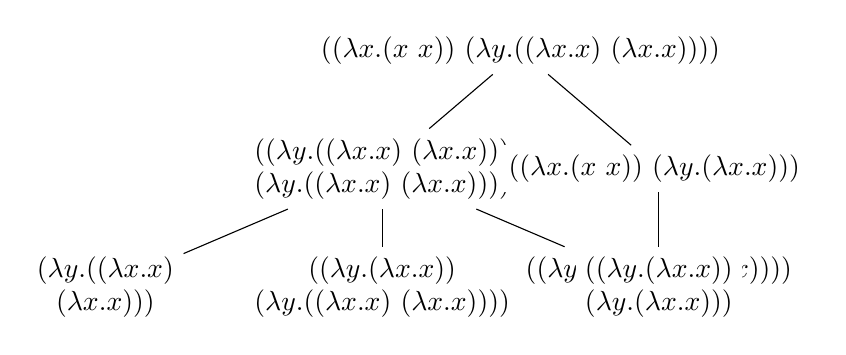
\begin{tikzpicture}[sibling distance=10em,
  every node/.style = {
     align=center,
    top color=white}]]
  \node {$((\lambda x.(x\ x))\ (\lambda y.((\lambda x.x)\ (\lambda x.x))))$}
    child { node {$((\lambda y.((\lambda x.x)\ (\lambda x.x)))$\\$(\lambda y.((\lambda x.x)\ (\lambda x.x))))$} 
      child {node{$(\lambda y.((\lambda x.x)$\\$(\lambda x.x)))$}}
      child {node{$((\lambda y.(\lambda x.x))$\\$(\lambda y.((\lambda x.x)\ (\lambda x.x))))$}}
      child {node{$((\lambda y.((\lambda x.x)\ (\lambda x.x))))$\\$(\lambda y.(\lambda x.x))$}}
      }
    child { node {$((\lambda x.(x\ x))\ (\lambda y.(\lambda x.x)))$
      }
      child {node {$((\lambda y.(\lambda x.x))$\\$(\lambda y.(\lambda x.x)))$}}
      };
      
\end{tikzpicture}
\end{center}
因此,一步关系$\rightarrow_{\mathbf{v}}$不满足菱形性质\par
因为基于\textbf{v}的一步关系的问题是由复制可约项的归约引起的,因此我们考虑一步关系$\rightarrow_{\mathbf{v}}$的拓展$\hookrightarrow_{\mathbf{v}}$,它可以并行收缩好几个不重叠的可约项。如果该拓展满足菱形性质,且它的自反传递闭包和$\rightarrow_{\mathbf{v}}$的相同,那么我们可以证明$\twoheadrightarrow_{\mathbf{v}}$归约的菱形性质。\par
并行拓展$\hookrightarrow_{\mathbf{v}}$的定义如下:
\begin{framed}
 $$
 \begin{array}{lcll}
  M & \hookrightarrow_{\mathbf{v}} & N & \text{如果}M=_\alpha N \\
  (o^n\ b_1\ \ldots b_\textbf{n}) & \hookrightarrow_{\mathbf{v}} & \sigma(o^n,\ b_1,\ldots b_\textbf{n}) & \text{如果定义了$\sigma(o^n,\ b_1,\ldots b_\textbf{n})$} \\
  ((\lambda X.M)\ N) & \hookrightarrow_{\mathbf{v}} & M'[X\leftarrow V] & \text{如果$M\hookrightarrow_{\mathbf{v}}M'$且$N\hookrightarrow_{\mathbf{v}}V$}\\
  (M\ N) & \hookrightarrow_{\mathbf{v}} & (M'\ N') & \text{如果$M\hookrightarrow_{\mathbf{v}}M'$且$N\hookrightarrow_{\mathbf{v}}N'$}\\
  (\lambda X.M) & \hookrightarrow_{\mathbf{v}} & (\lambda x.M') & \text{如果$M\hookrightarrow_{\mathbf{v}}M'$}\\
  (o^n\ M_1\ \ldots M_\textbf{n}) & \hookrightarrow_{\mathbf{v}} & (o^n\ M'_1\ \ldots M'_\textbf{n}) & \text{如果对$i\in[1,n]$有$M_i\hookrightarrow_{\mathbf{v}}M'_i$}
 \end{array}
 $$
\end{framed}
这个关系满足菱形性质。
\begin{Theorem}[$\hookrightarrow_{\mathbf{v}}$的菱形性质]
 如果$L\hookrightarrow_{\mathbf{v}}M$且$L\hookrightarrow_{\mathbf{v}}N$,那么存在表达式K使$M\hookrightarrow_{\mathbf{v}}K$且$M\hookrightarrow_{\mathbf{v}}K$。
\end{Theorem}
\begin{adjustwidth}{20pt}{20pt}
 \textbf{定理4.6的证明}:基于$L\hookrightarrow_{\mathbf{v}}$证明树结构的归约进行证明。
 \begin{itemize}
  \item 奠基步骤
  \begin{itemize}
   \item \textbf{当$L=_\alpha M$时}\\
   令$K=N$,命题得证。
   \item \textbf{当$L=(o^n\ b_1\ldots\ b_\textbf{n}),M=\sigma(o^n,b_1,\ldots b_\textbf{n})$时}\\
   因为$\sigma$是函数,所以没有其他可能对L的归约。令$K=N=M$即可。
  \end{itemize}
  \item 归纳步骤
  \begin{itemize}
   \item \textbf{当$L=((\lambda X.M_0)\ L_1), M=M'_0[X\leftarrow V],M_0\hookrightarrow_{\mathbf{v}}M'_0,L_1\hookrightarrow_{\mathbf{v}}V$时}\\
   $L\hookrightarrow_{\mathbf{v}}N$有两种可能的归约路径:要么应用的两部分各自完全分开归约,要么该应用使用$\beta_{\mathbf{v}}$归约:
    \begin{itemize}
     \item \textbf{当}$L=((\lambda X.M_0\ L_1)), N=((\lambda X.M''_0)\ L''_1), M_0\hookrightarrow_{\mathbf{v}}M''_0, L_1\hookrightarrow_{\mathbf{v}}L''_1$\textbf{时}\\
     在这种情况下$M_0$,$M'_0$和$M''_0$满足归约假设的前项,$L_1$,$V$和$L''_1$也满足。因此,存在补全两个菱形上半部分的表达式$K_0$和$K_1$。我们如果知道替换和并行归约是可交换的,就可以根据$((\lambda X.M''_0)\ L''_1)\hookrightarrow_{\mathbf{v}}K_0[X\leftarrow K_1]$和$M=M'_0[X\leftarrow V]\hookrightarrow_{\mathbf{v}}K'[X\leftarrow K_1]$得到$K=K_0[X\leftarrow K_1]$。
      \item \textbf{当$L=((\lambda X.M_0)\ L_1), M=M''_0[X\leftarrow V'],M_0\hookrightarrow_{\mathbf{v}}M''_0,L_1\hookrightarrow_{\mathbf{v}}V'$时}\\
      就像在第一个子情况中,$M_0$,$M''_0$和$M'''_0$以及$L_1$,$V$和$L''_1$决定的菱形的上半部分。根据归纳假设,每个都产生了两个菱形的下半部分和相关项$K_0$和$K_1$。再者,如果替换和并行归约是可交换的,则令$K=K_0[X\leftarrow V]$即可得出该子情况。
    \end{itemize}
  为了补全这个情况,我们必须证明其交换性质。不过我们推迟这个证明,因为还有其他的情况依赖它,见引理4.7。
  \item \textbf{当}$L=(L_1\ L_2), M= (M_1\ M_2), L_i\hookrightarrow_{\mathbf{v}}M_i$\textbf{时}
  和前一个情况相同。
  \item \textbf{当}$L=(o^n\ L_1\ldots L_\textbf{n})$,$M=(o^n\ M_1\ldots M_\textbf{n})$,$ L_i\hookrightarrow_{\mathbf{v}} M_i$\textbf{时}\\
  有两种情况:
  \begin{itemize}
   \item \textbf{当}$L_1=b_1,\ldots L_\textbf{n}=b_\textbf{n}$,$N=\sigma(o^n,b_1,\ldots b_\textbf{n})$\textbf{时}\\
   那么$M=L$且$K=N$
   \item \textbf{当}$N=(o^n\ N_1\ldots N_\textbf{n})$,$L_i\hookrightarrow_{\mathbf{v}} N_i$\textbf{时}\\
   一个n折的归纳假设可以得出结论。
  \end{itemize}
  \item \textbf{当}$L=(\lambda X.L_0)$,$M=(\lambda X.M_0)$,$L_0\hookrightarrow_{\mathbf{v}} M_0$\textbf{时}\\
  N唯一的可能是$N=(\lambda X,N_0)$且$L_0\hookrightarrow_{\mathbf{v}} N_0$。那么归纳假设适用于$L_0$,$M_0$和$N_0$且产生表达式$K_0$,有$K=(\lambda X.K_0)$。
  \end{itemize}
 \end{itemize}
\end{adjustwidth}
为了完成上述证明,我们需要证明表达式关于并行归约相关的表达式中的替换不影响归约步骤。
\begin{Lemma}
 如果$M\hookrightarrow_{\mathbf{v}}M'$且$N\hookrightarrow_{\mathbf{v}}N'$那么$M[X\leftarrow N]\hookrightarrow_{\mathbf{v}} M'[X\leftarrow N']$。
\end{Lemma}
\begin{adjustwidth}{20pt}{20pt}
\textbf{引理4.7的证明}:根据$M\hookrightarrow_{\mathbf{v}}M'$证明树的归约进行证明:
\begin{itemize}
 \item 奠基步骤
 \begin{itemize}
  \item \textbf{当$M=_\alpha M'$时}\\
  在这种特殊情况下,这个命题实际上等同于如果$N\hookrightarrow_{\mathbf{v}} N'$,那么$M[X\leftarrow N]\hookrightarrow_{\mathbf{v}} M[X\leftarrow N']$。这个特殊结论的证明是基于M结构的归约。我们将这个证明留作练习。
  \item \textbf{当$M=(o^n b_1\ldots b_\textbf{n})$,$M'=\sigma(o^n,b_1,\ldots b_\textbf{n})$时}\\
  $M$和$M'$是封闭的,所以$M[X\leftarrow N]=M$且 $M'[X\leftarrow N]=M'$,而且我们已经知道$M\hookrightarrow_{\mathbf{v}} M'$。
 \end{itemize}
 \item 归纳步骤
 \begin{itemize}
  \item \textbf{当$M=((\lambda X_0.M_0)\ L_0)$,$M'=M'_0[X_0\leftarrow V]$,$M_0\hookrightarrow_{\mathbf{v}} M'_0$,$L_0\hookrightarrow_{\mathbf{v}} V$时。}\\
  根据归纳,$M_0[X\leftarrow N]\hookrightarrow_{\mathbf{v}} M'_0[X\leftarrow N']$且$L_0[X\leftarrow N]\hookrightarrow_{\mathbf{v}} V[X\leftarrow N']$。因此:
  $$
  \begin{array}{lcll}
   M[X\leftarrow N] &= & ((\lambda X_0.M_0[X\leftarrow N])\ L_0[X\leftarrow N]) \\
   &\hookrightarrow_{\mathbf{v}} & M'_0[X\leftarrow N'][X_0\leftarrow V[X\leftarrow N']] \\
   &=& M'_0[X_0\leftarrow V][X\leftarrow N'] & (\dagger)\\
   &=_\alpha&M'[X\leftarrow N']
  \end{array}
  $$
  等式$(\dagger)$是替换函数的基本性质。我们将这一步骤留作练习。
  \item \textbf{当$M=(M_1\ M_2)$,$M'=(M'_1\ M'_2)$,$M_i\hookrightarrow_{\mathbf{v}} M'_i$时}\\
  根据归约,对$i=1$和$i=2$都有$M_i[X\leftarrow N]\hookrightarrow_\v M'_i [X\leftarrow N']$,因此有\\
  $$
  \begin{array}{lcl}
   M[X\leftarrow N] & = & (M_1[X\leftarrow N]\ M_2[X\leftarrow N])\\
   & \hookrightarrow_{\mathbf{v}} &(M'_1[X\leftarrow N]\ M'_2[X\leftarrow N])\\
   & \hookrightarrow_{\mathbf{v}} &(M'_1[X\leftarrow N']\ M'_2[X\leftarrow N'])\\
   & = & (M'_1\ M'_2)[X\leftarrow N']\\
   & = & M'[X\leftarrow N']
  \end{array}
  $$\\
  所以论题得证。
  \item \textbf{当$M=(o^n\ M_1\ldots\ M_\textbf{n})$,$M'=(o^n\ M'_1\ldots\ M'_\textbf{n})$,$M_i\hookrightarrow_{\mathbf{v}} M'_i$时}\\
  和上面的情况相同。
  \item \textbf{当$M=(\lambda X.M_0)$,$M=(\lambda X.M'_0)$,$M_0\hookrightarrow_{\mathbf{v}} M'_0$时}\\
  和上面的情况相同。
  
 \end{itemize}
\end{itemize}
\end{adjustwidth}
\lianxi{练习4.3.}证明如果$N\hookrightarrow_\v N'$,那么$M[X\leftarrow N]\hookrightarrow_\v M[X\leftarrow N']$。\\\\
\lianxi{练习4.4.}证明如果$X\not\in\mathcal{FV}(L)$,那么$$K[X\leftarrow L][X'\leftarrow M[X\leftarrow L]]=_\alpha K[X'\leftarrow M][X\leftarrow L]$$\\\\
\lianxi{练习4.5.}证明并行关系$\hookrightarrow_\v$的传递自反闭包和$\twoheadrightarrow_\v$相同。这个结论连同定理4.6的证明,可支持定理4.5的证明。
\section{观察等价性}
除了程序求值器,程序转换在编程实践和编程语言实现时都发挥了很重要的作用。例如,如果M是一个程序,如果我们认为程序N的计算行为和M相同但是计算得更快,那么我们就要证明M是否真的可以和N互换。ISWIM为这个问题的一个特殊案例提供了一个清晰的方案:如果两个表达式都是完整的程序且我们知道$M=_\mathbf{v}N$,那么我们可得$eval_\v(M) = eval_\v(N)$且可知能够使用M替换N。\par
但是一般来说,M和N是一些程序中的子表达式,而且我们可能不能将它们独立求值。因此,我们真正需要的是一个可以解释什么时候表达式是“功能性等价”的一般性关系。\par
为了理解“功能性等价”的概念,我们必须回想程序的使用者仅能“观察”到输出,也对输出最感兴趣。程序员通常不知道程序文本或任何关于文本的概念。换句话说,这样的观察者将程序当作使用某种未知规则而产生某个值的黑箱。因此,表达式的影响自然是其作为程序一部分所产生的影响。甚至更进一步地说,两个开放表达式的比较可以归约成是否存在一种辨别表达式影响的方法的问题。或者更正式地说,如果两个表达式具有相同的影响,那么从外部的观察者的视角看来,它们是可以交换的。\par
在继续之前,我们需要表达式上下文的概念。下面的文法C定义了一种贴近表达式的集合。他们不是严格的表达式,因为C的每个元素都在其中一个子表达式上存在一个\textbf{洞},记为$[]$。
\begin{framed}
 $$
 \begin{array}{lcl}
  C & = & []\\
  & | & (\lambda X.C)\\
  & | & (C\ M) \\
  & | & (M\ C) \\
  & | & (o^n\ M\ \ldots\ M\ C\ M\ \ldots\ M)\\
 \end{array}
$$
$$
C[M]\text{意味着“将$C$中的$[]$替换为$M$”}
$$
\end{framed}
例如,$(\lambda x.[])$和$(+\ 1\ ((\lambda x.^\lceil 0^\rceil)\ []))$是C的元素,且
$$
\begin{array}{lcl}
(\lambda x.[])[(\lambda y.x)] &=&  (\lambda x.(\lambda y.x))\\
(+\ 1\ ((\lambda x.^\lceil 0^\rceil)\ []))[(z\ ^\lceil 12^\rceil)] & = &(+\ 1\ ((\lambda x.^\lceil 0^\rceil)\ (z\ ^\lceil 12^\rceil)))
\end{array}
$$
与替换不同的是,填补一个上下文洞可以捕捉变量。\par
根据这个上下文定义,我们可以表示观察等价性的概念,两个表达式M和N是\textbf{观察等价}的,当且仅当它们在所有上下文C中都没有差别,记为$M\simeq_\v N$。
\begin{framed}
 $$
 M\simeq_\v N\quad \text{如果对所有的$C$,有}eval_\v(C[M])=eval_\v(C[N])
 $$
\end{framed}
这个定义暗示了如果$M\simeq_\v N$,那么$eval_\v(C[M])$和$eval_\v(C[N])$对任何C,要么都被定义了,要么都没被定义。\par
观察等价性明显的拓展了在$eval_\v$意义上的程序等价性。如果程序M和N是观察等价的,那么他们空集上下文中就是程序,所以$eval_\v(M)=eval_\v(N)$。但是至少我们也希望在等价功能表达式理论中获得这些信息了。如其名所示,观察等价性是一个等价关系。最后,如果两个表达式是观察等价的,那么将它们嵌入到上下文中,也会产生等价表达式。毕竟被加入的部分是恒等的且不应该影响表达式在程序输出上可能产生的效果。简而言之,观察等价性是一个\textbf{同余关系},也就是说,它基于上下文的闭包也是一个等价关系。
\begin{Theorem}
 对任何表达式M、N和L都有
 \begin{enumerate}
  \item $M\simeq_\v M$
  \item 如果$L\simeq_\v M$且$M\simeq_\v N$,那么$L\simeq_\v N$
  \item 如果$L\simeq_\v M$,那么$M\simeq_\v L$
  \item 如果$M\simeq_\v N$,那么对于所有的上下文C都有$C[M]\simeq_\v C[N]$
 \end{enumerate}
\end{Theorem}
\begin{adjustwidth}{20pt}{20pt}
 \textbf{定理4.8的证明:}通过3可知第1点是平凡的。至于第四点,假设$M\simeq_\v N$且令$C'$为一个任意的上下文。那么$C'[C]$是M和N的上下文。因此根据假设$M\simeq_\v N$可得
 $$
 eval_\v(C'[C[M]]) = eval_\v(C'[C[N]])
 $$
 该等式是我们必须证明的。
\end{adjustwidth}
实际上观察等价性是满足我们直观标准的表达式的最大同余关系。
\begin{Theorem}
 令$\R$是同余关系,且对表达式M、N有,通过$M\ \R\ N$可得$eval_\v(M)=eval_\v(N)$。如果$M\ \R\ N$,那么$M\simeq_\v N$。
\end{Theorem}
\begin{adjustwidth}{20pt}{20pt}
 \textbf{定理4.9的证明}:我们假设$M\not\simeq_\v N$且显示$M\ \not\R\ N$。根据假设存在一个分离的上下文C。也就是说,$eval_\v(C[M])\neq eval_\v(C[N])$。因此,$C[M]\ \not\R\ C[N]$。因为$\R$被假设是一个同余关系,我们不能得出$M\equiv N$,因为这是矛盾的。
\end{adjustwidth}
这个命题证明了观察等价性是表达式最基本、最基础的同余关系。所有其他的关系仅仅接近观察等价性定义表达式是所需要的精确性。就观察定价性而言,它也遵循ISWIM的稳固性命题。但遗憾的是,它也是不完整的,这个演算不能证明所有的观察等价关系。
\begin{Theorem}[稳固性,不完整性]
 如果我们能证明 $M=_\v N$,那么$M\simeq_\v N$。但是$M\simeq_\v N$并不意味着能推出$M=_\v N$。
\end{Theorem}
\begin{adjustwidth}{20pt}{20pt}
 \textbf{定理4.10的证明}:根据定义,$=_\v$是同余关系。此外$eval_\v$是基于$=_\v$定义的,也就是说如果$M=_\v N$则$eval_\v(M) = eval_\v(N)$。\\
 对于相反的情况,我们可以给出一个反例并简述该反例的证明。例如表达式$(\Omega\ (\lambda x.x))$和$\Omega$,其中$\Omega=((\lambda x.(x\ x))\ (\lambda x.(x\ x))$,这两个表达式都是发散的且观察等价的。但是二者都仅归约到自身,因此不能被证明是关系$=_\v$。
\end{adjustwidth}
我们仍然缺少一些工具去完成不完全性定理的证明。我们在下一章拓展了关于ISWIM的一些拔高于基本知识的内容,同时也将继续这个证明。\\\\
\lianxi{练习4.6.}考虑下列求值函数$eval_0$,以及其相关的观察等价关系$\simeq_0$:
$$
\begin{array}{ll}
 eval_0(M)=\mathbf{value} & \text{如果对某些V有}M=_\v V\\
 M \simeq_0 N & \text{如果对所有的C,有}eval_0(C[M])=eval_0(C[N])
\end{array}
$$
$M\simeq_0 N$能推导出任何关于$M\simeq_\v N$的结论吗?简述你答案的理由。
\section{历史}
在二十世纪60年代中期的一系列论文中[5],Landin详述了两个关于编程语言的重要发现。第一,他认为所有的编程语言都有一套用于详细描述计算的共享基元集合\footnote{译者注:原文为“a basic set of facilities”},但是对数据和数据元的选择有所不同。基本的基元集合包括命名、过程、应用、异常机制、可变数据结构以及可能的其他形式的非局部控制。数值应用语言通常包含多种形式的数值常量和大量的数值元集合,然而字符串操作语言一般提供高效的字符串匹配和操作元。\par
第二,他极力主张程序员和语言实现者一样,都应把编程语言当成算数与代数的一种高级的符号化形式。因为我们都习惯于使用数值、布尔,甚至我们从幼儿园到高中期间学习的更为复杂的数据结构来进行计算,这些计算也应该易于被程序计算。程序求值、多种形式的程序编辑、程序转换和优化都只是不同的、更为复杂的计算形式。这类计算处理关于程序或程序片段的问题,而不是简单的算数表达式。\par
Landin定义了编程语言ISWIM。他的设计基于丘奇的$\lambda$演算——从Landin认为程序过程的核心作用是作为所有语言的共享基元的观点看,这是一个自然会想到的着手点。但是,为了支持基本数据以及赋值和控制结构的相关元,Landin通过恰当的结构拓展了$\lambda$演算。他通过一种抽象机器指定了这个拓展语言的语义,因为他不知道如何将$\lambda$演算的等价理论拓展到完整的编程语言理论中。实际上,事实证明$\lambda$演算甚至不能解释纯函数式子语言的语义,因为ISWIM总是对程序过程的参数进程求值。因此,Landin没有完成自己着手去做的事情,也就是没有定义理想化的所有编程语言的核心以及定义其语义的等价演算。\par
自二十世纪70年代中叶Plotkin关于抽象机器和等价演算的关系的工作开始后,就有大量的研究者,包括Felleisen,Mason,Talcott以及他们的合作者,补充Landin研究中的不足。Plotkin的工作涵盖了ISWIM的基本函数式子语言,这需要$\lambda$演算的按值调用变量的定义。Felleisen和他的合作者根据若干种可解释不同类型的必要语言基元的公理,拓展了等价性理论。Mason和Talcott研究了在完全类ISWIM语言作为一种程序验证和程序转换的工具的等价性理论的应用。\par
虽然ISWIM没有成为广泛使用的语言,但是ISWIM的哲学仍存在于现代编程语言中,尤其是Scheme和ML语言中,而其语言分析和设计方法基本应用于所有编程语言中。本书的另一个目标是说明等价性理论的设计、分析和应用,例如在编程语言的设计和分析背景下的$\lambda$演算。
\end{document}